% Options for packages loaded elsewhere
\PassOptionsToPackage{unicode}{hyperref}
\PassOptionsToPackage{hyphens}{url}
\PassOptionsToPackage{dvipsnames,svgnames,x11names}{xcolor}
%
\documentclass[
]{article}
\usepackage{amsmath,amssymb}
\usepackage{iftex}
\ifPDFTeX
  \usepackage[T1]{fontenc}
  \usepackage[utf8]{inputenc}
  \usepackage{textcomp} % provide euro and other symbols
\else % if luatex or xetex
  \usepackage{unicode-math} % this also loads fontspec
  \defaultfontfeatures{Scale=MatchLowercase}
  \defaultfontfeatures[\rmfamily]{Ligatures=TeX,Scale=1}
\fi
\usepackage{lmodern}
\ifPDFTeX\else
  % xetex/luatex font selection
\fi
% Use upquote if available, for straight quotes in verbatim environments
\IfFileExists{upquote.sty}{\usepackage{upquote}}{}
\IfFileExists{microtype.sty}{% use microtype if available
  \usepackage[]{microtype}
  \UseMicrotypeSet[protrusion]{basicmath} % disable protrusion for tt fonts
}{}
\makeatletter
\@ifundefined{KOMAClassName}{% if non-KOMA class
  \IfFileExists{parskip.sty}{%
    \usepackage{parskip}
  }{% else
    \setlength{\parindent}{0pt}
    \setlength{\parskip}{6pt plus 2pt minus 1pt}}
}{% if KOMA class
  \KOMAoptions{parskip=half}}
\makeatother
\usepackage{xcolor}
\usepackage[margin=1in]{geometry}
\usepackage{graphicx}
\makeatletter
\newsavebox\pandoc@box
\newcommand*\pandocbounded[1]{% scales image to fit in text height/width
  \sbox\pandoc@box{#1}%
  \Gscale@div\@tempa{\textheight}{\dimexpr\ht\pandoc@box+\dp\pandoc@box\relax}%
  \Gscale@div\@tempb{\linewidth}{\wd\pandoc@box}%
  \ifdim\@tempb\p@<\@tempa\p@\let\@tempa\@tempb\fi% select the smaller of both
  \ifdim\@tempa\p@<\p@\scalebox{\@tempa}{\usebox\pandoc@box}%
  \else\usebox{\pandoc@box}%
  \fi%
}
% Set default figure placement to htbp
\def\fps@figure{htbp}
\makeatother
\setlength{\emergencystretch}{3em} % prevent overfull lines
\providecommand{\tightlist}{%
  \setlength{\itemsep}{0pt}\setlength{\parskip}{0pt}}
\setcounter{secnumdepth}{-\maxdimen} % remove section numbering
% definitions for citeproc citations
\NewDocumentCommand\citeproctext{}{}
\NewDocumentCommand\citeproc{mm}{%
  \begingroup\def\citeproctext{#2}\cite{#1}\endgroup}
\makeatletter
 % allow citations to break across lines
 \let\@cite@ofmt\@firstofone
 % avoid brackets around text for \cite:
 \def\@biblabel#1{}
 \def\@cite#1#2{{#1\if@tempswa , #2\fi}}
\makeatother
\newlength{\cslhangindent}
\setlength{\cslhangindent}{1.5em}
\newlength{\csllabelwidth}
\setlength{\csllabelwidth}{3em}
\newenvironment{CSLReferences}[2] % #1 hanging-indent, #2 entry-spacing
 {\begin{list}{}{%
  \setlength{\itemindent}{0pt}
  \setlength{\leftmargin}{0pt}
  \setlength{\parsep}{0pt}
  % turn on hanging indent if param 1 is 1
  \ifodd #1
   \setlength{\leftmargin}{\cslhangindent}
   \setlength{\itemindent}{-1\cslhangindent}
  \fi
  % set entry spacing
  \setlength{\itemsep}{#2\baselineskip}}}
 {\end{list}}
\usepackage{calc}
\newcommand{\CSLBlock}[1]{\hfill\break\parbox[t]{\linewidth}{\strut\ignorespaces#1\strut}}
\newcommand{\CSLLeftMargin}[1]{\parbox[t]{\csllabelwidth}{\strut#1\strut}}
\newcommand{\CSLRightInline}[1]{\parbox[t]{\linewidth - \csllabelwidth}{\strut#1\strut}}
\newcommand{\CSLIndent}[1]{\hspace{\cslhangindent}#1}
\usepackage[left]{lineno}
\linenumbers
\usepackage{fancyhdr}
\usepackage{bookmark}
\IfFileExists{xurl.sty}{\usepackage{xurl}}{} % add URL line breaks if available
\urlstyle{same}
\hypersetup{
  pdftitle={Flexibility training does not increase behavioral diversity of Florida scrub-jays},
  pdfauthor={McCune, KB1,2; Barve, S3},
  colorlinks=true,
  linkcolor={Maroon},
  filecolor={Maroon},
  citecolor={Blue},
  urlcolor={blue},
  pdfcreator={LaTeX via pandoc}}

\title{Flexibility training does not increase behavioral diversity of
Florida scrub-jays}
\author{\href{https://www.kelseymccune.com/}{McCune,
KB}\textsuperscript{1,2} \and \href{http://www.sahasbarve.com/}{Barve,
S}\textsuperscript{3}}
\date{2026-03-17}

\begin{document}
\maketitle

Open\ldots{}

\includegraphics[width=0.05\linewidth,height=\textheight,keepaspectratio]{logoOpenAccess.png}
access

\includegraphics[width=0.05\linewidth,height=\textheight,keepaspectratio]{logoOpenCode.png}
\href{https://github.com/ManyIndividuals/ManyIndividuals/blob/main/Files/rrs/mi1.Rmd}{code}

~

\subparagraph{Affiliations:}\label{affiliations}

\begin{enumerate}
\def\labelenumi{\arabic{enumi})}
\tightlist
\item
  Institute for Social, Behavioral and Economic Research, University of
  California Santa Barbara, Santa Barbara, CA, USA
\item
  College of Forestry, Wildlife and Environment, Auburn University,
  Auburn, AL, USA
\item
  Archbold Biological Station, Venus, FL, USA.
\end{enumerate}

\emph{Corresponding author:
\href{mailto:kelseybmccune@gmail.com}{\nolinkurl{kelseybmccune@gmail.com}}}

~

\textbf{This is a post-study manuscript of the registered report that
has been pre-study peer reviewed and received an In Principle Acceptance
on 8 Sep 2022 by:}

Chris Chambers (2022) The role of behavioural flexibility in promoting
resilience to human environmental impacts. \emph{Peer Community in
Registered Reports}.
\url{https://rr.peercommunityin.org/articles/rec?id=200}. Reviewers:
Gloriana Chaverri, Vedrana Šlipogor, and Alizée Vernouillet


\includegraphics[width=0.5\linewidth,height=\textheight,keepaspectratio]{logoPCIRR.png}

\emph{See the reproducible manuscript
(\href{https://github.com/ManyIndividuals/ManyIndividuals/blob/573b4b5802550f47f246fb8b71c8efc4f853445c/Files/rrs/mi1.Rmd}{Rmd})
version for the code}

~

\newpage

\section{\texorpdfstring{\textbf{ABSTRACT}}{ABSTRACT}}\label{abstract}

Human modifications of environments are expanding, causing global
changes that other species must adjust to or suffer from. Behavioral
flexibility (hereafter `flexibility') could be key to coping with rapid
change. Behavioral research can contribute to conservation by
determining which behaviors can predict the ability to adjust to human
modified environments and whether these can be manipulated. When
research that manipulates behavior in a conservation context occurs, it
primarily trains a specific behavior to address one potential threat
improve individual success in the wild. However, training a domain
general cognitive ability, such as flexibility, has the potential to
change a whole suite of behaviors, which could have a larger impact on
influencing success in adjusting to human modified environments. This
project asks whether flexibility can be increased by experimentally
increasing environmental heterogeneity and whether such an increase can
help species succeed in human modified environments. We explore whether
it is possible to take insights from highly divergent species and apply
them to address critical conservation challenges. This pushes the limits
in terms of understanding how conserved these abilities may be and to
what extent they can be shaped by the environment. We aim to 1) conduct
flexibility interventions in flexible species that are successful in
human modified environments (California scrub-jays or blue jays) to
understand how flexibility relates to success; and 2) implement these
interventions in a vulnerable species (Florida scrub-jays) to determine
whether flexibility as a generalizable cognitive ability can be trained
and whether such training improves success in human-modified
environments. This research will significantly advance our understanding
of the causes and consequences of flexibility, linking behavior to
environmental change, cognition, and success in human modified
environments through a comparative framework.

\section{\texorpdfstring{\textbf{REGISTERED REPORT
DETAILS}}{REGISTERED REPORT DETAILS}}\label{registered-report-details}

\begin{itemize}
\tightlist
\item
  \textbf{Level of bias = 6:} This registered report was written (Jul
  2021-May 2022), and revised after round one of peer review at Peer
  Community in Registered Reports (Jul 2022) prior to collecting any
  data.
\item
  \textbf{Programmatic registered report:} This is one of three Stage 2
  articles that will result from the original, comprehensive Stage 1
  registered report: one for toutouwai, one for grackles, and one for
  jays (this current manuscript).
\item
  \textbf{Deviations from the Stage 1 registered report:} We were unable
  to sample disturbance-resilient blue jays or California scrub-jays and
  so we cannot address J.Q2 (one of four specific research questions) at
  this time. However, to begin to test the question of whether behavior
  relates to success in human-modified environments, we conducted an
  unregistered analysis comparing behavior of Florida scrub-jays (FLSJ;
  a species that is overall disturbance-sensitive) that were persisting
  in suburban areas to FLSJ in natural habitat managed without human
  disturbance.
\end{itemize}

\section{\texorpdfstring{\textbf{INTRODUCTION}}{INTRODUCTION}}\label{introduction}

Human modified environments are expanding (Goldewijk, 2001; X. Liu et
al., 2020; Wu et al., 2011), causing global changes that other species
must adjust to or suffer from (Alberti, 2015; Chejanovski et al., 2017;
Ciani, 1986; Federspiel et al., 2017). Behavioral flexibility (hereafter
`flexibility') could be key for adjusting to such change: individuals
interact with their environment through behavior, making it crucial to
an ecologically valid understanding of how species adjust to
environmental changes (Lee \& Thornton, 2021). One of the top priorities
for behavioral research to maximize conservation progress is to
determine which cognitive abilities and behaviors can predict the
ability to adjust to human modified environments and whether these can
be manipulated (Moseby et al., 2016). The rare research that manipulates
behavior in a conservation context usually focuses on training specific
behaviors (for example, predator recognition through predator exposure)
to improve individual success in the wild (Jolly et al., 2018; Moseby et
al., 2012; Ross et al., 2019; West et al., 2018; see review in Tetzlaff
et al., 2019). However, training a general cognitive ability, such as
flexibility -- the ability to rapidly adapt behavior to changes through
learning throughout the lifetime (see the theory behind this definition
in Mikhalevich et al., 2017) -- has the potential to change a whole
suite of behaviors and more broadly influence success in adjusting to
human modified environments. Recent evidence supports this hypothesis:
as far as we are aware, our previous research in the great-tailed
grackle was the first to show that flexibility can be manipulated using
serial reversal learning of color preferences, and that the manipulated
individuals were more flexible during foraging (Logan et al., 2025), in
a different experimental context (locus switching on a puzzlebox) as
well as being more innovative (solved more loci on a puzzlebox) (Logan
et al., 2023).

Environments where informational cues about resources vary in a
heterogeneous (but non-random) way across space and time are
hypothesized to open a pathway for species to functionally detect and
react to such cues via flexibility (Mikhalevich et al., 2017). Human
modified environments likely provide a different set of informational
cues that vary heterogeneously across space and time, and the species
that are successful in such environments are likely those who are able
to detect and track such cues. Because heterogeneous environments are
hypothesized to select for flexibility (Wright et al., 2010), we expect
that exposing individuals to experimentally increased environmental
heterogeneity will train individuals to be more flexible, which will
then increase their success in such environments (Fig. 1). Success can
relate to any number of variables regarding the usage of and investment
in resources and response to threats, from improved foraging efficiency
to increased dispersal and survival within human modified environments,
to placing nests in more protective locations. Whether a measure of
success is predicted to relate to flexibility depends on what is already
known about the particular population and their particular environment.

~

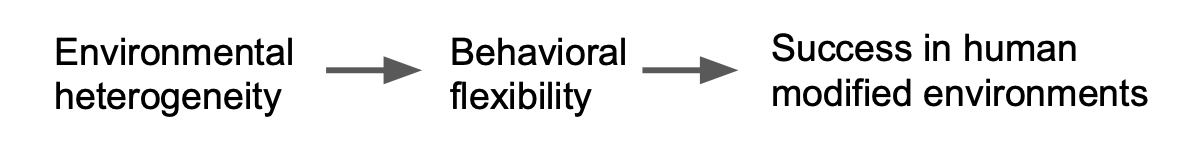
\includegraphics[width=1\linewidth,height=\textheight,keepaspectratio]{mi1Figdag.png}
\textbf{Figure 1.} The theory behind this research illustrated by a
directed acyclic graph (DAG), which is a theoretical model of the causal
relationships among the key variables in our investigation. Based on the
theoretical background provided by Mikhalevich et al. (2017), we assume
that more heterogeneity causes more flexibility, which then causes more
success in human modified environments.

~

This investigation asks whether a method of experimentally increasing
environmental heterogeneity through serial reversal learning leads to
increased behavioral flexibility and greater fitness in human modified
environments. Serial reversal learning tasks have been performed with a
wide diversity of species (birds: Bond et al., 2007; bumblebees: Strang
\& Sherry, 2014; stingrays: Daniel \& Schluessel, 2020). There is
variation across individuals and species in their performance, however
almost all previous studies show that individuals improve their
flexibility if the reversal intervention is given multiple times in
sequence (rats: Mackintosh et al., 1968; guppies: Lucon-Xiccato \&
Bisazza, 2014; poison frogs: Y. Liu et al., 2016; grackles: Logan et
al., 2023). We aim to conduct a flexibility intervention in species that
are successful in human modified environments (California scrub-jays or
blue jays) to understand how flexibility relates to success, and
implement these interventions in a vulnerable species (Florida
scrub-jays).

While we do not examine the potential spread of the post-manipulation
success behaviors from manipulated individuals to individuals that are
not involved in our studies, we acknowledge that this is a possibility
worthy of future investigation. Manipulating the flexibility of a few
individuals could have population-level effects because significant
research on social information use in birds (e.g., Valente et al., 2021)
demonstrates the potential for the manipulated behavior to disseminate
to conspecifics (for example, if manipulated individuals are faster at
locating new resources, which could attract the attention of
conspecifics, or if unmanipulated individuals copy the manipulated
individuals' nesting or foraging locations). Indeed, there is evidence
for social learning in the focal species for this investigation (K. B.
McCune et al., 2022; Midford et al., 2000). In the event that social
learning is not used by a given population to spread the behaviors of
manipulated individuals, investing in the training of specific
individuals to increase their success in the wild could still have
conservation impacts. In some cases, it is possible to train many
individuals in a population or a species because there are not many
individuals left (Greggor et al., 2021). It is also possible to train
all individuals involved in a conservation management event such as a
translocation (Greggor et al., 2021). Therefore, there can still be
significant population consequences even if each individual needs to be
trained to achieve the goal.

This comparative approach will ultimately reveal the role of behavioral
flexibility in adaptation to environmental change and whether there is a
causal relationship between this general cognitive trait and behavioral
interactions with human-modified environments, such as foraging and
habitat use. Our previous research on great-tailed grackles provided
support that this causal relationship does exist in a generalist,
invasive species. However, the research presented here will evaluate the
generalizability of this technique across distinct species
differentially affected by anthropogenic change. Consequently, the
results from this research will substantially advance our understanding
of the causes and consequences of flexibility, linking behavior to
environmental change, cognition, and success in human modified
environments to facilitate conservation of declining species.

\section{\texorpdfstring{\textbf{RESEARCH
QUESTIONS}}{RESEARCH QUESTIONS}}\label{research-questions}

\subsection{Can behavioral flexibility in individuals be increased by
increasing environmental heterogeneity? If so, does increased
flexibility help individuals succeed in human modified
environments?}\label{can-behavioral-flexibility-in-individuals-be-increased-by-increasing-environmental-heterogeneity-if-so-does-increased-flexibility-help-individuals-succeed-in-human-modified-environments}

\textbf{Prediction 1:} Flexibility can be increased in individuals and
such an increase \textbf{improves the likelihood of success in human
modified environments}. This would indicate that the abilities involved
in tracking changing resources in the environment are the same as or
related to the abilities involved in succeeding in human modified
environments. It would also indicate that flexibility is trainable and
that such training could be a useful conservation tool for threatened
and endangered species.

\textbf{Prediction 1 alternative 1:} Flexibility can be increased in
individuals, but such an increase \textbf{does not improve the
likelihood of success} in human modified environments. This would
indicate that species associated with human modified environments form
this association for reasons other than their flexibility, and that
threatened species are likely not very successful in human modified
environments for reasons unrelated to their ability to change their
behavior with changing circumstances. An alternative could be that the
changes induced by the increase in flexibility do not persist for
sufficiently long times to make a difference on the subsequent
likelihood of success (changes in great-tailed grackles were still
present for four weeks after the manipulation and longer time periods
were not attempted so the threshold is unknown Logan et al., 2022).

\textbf{Prediction 1 alternative 2:} Flexibility can be increased in
some populations, but not others. This would indicate that
\textbf{flexibility manipulations may not work for all populations}, and
that the effectiveness of such experiments should first be tested in the
population of interest before including such an intervention in a
conservation plan. If flexibility is not manipulatable in threatened
populations, this would indicate that they are likely not very
successful in human modified environments because of their inability to
change their behavior with changing circumstances, and that flexibility
is not trainable. If flexibility is not manipulatable in populations
that are successful in human modified environments, this could indicate
that they might have used flexibility in the past when originally
forming the association, but the need to maintain flexibility in their
repertoire is no longer necessary (Wright et al., 2010). In populations
where flexibility is not manipulatable, this would indicate that the
abilities involved in tracking changing resources in the environment are
independent of the abilities involved in succeeding in human modified
environments.

\newpage

\subsection{Population-specific background and tailored research
questions}\label{population-specific-background-and-tailored-research-questions}

~

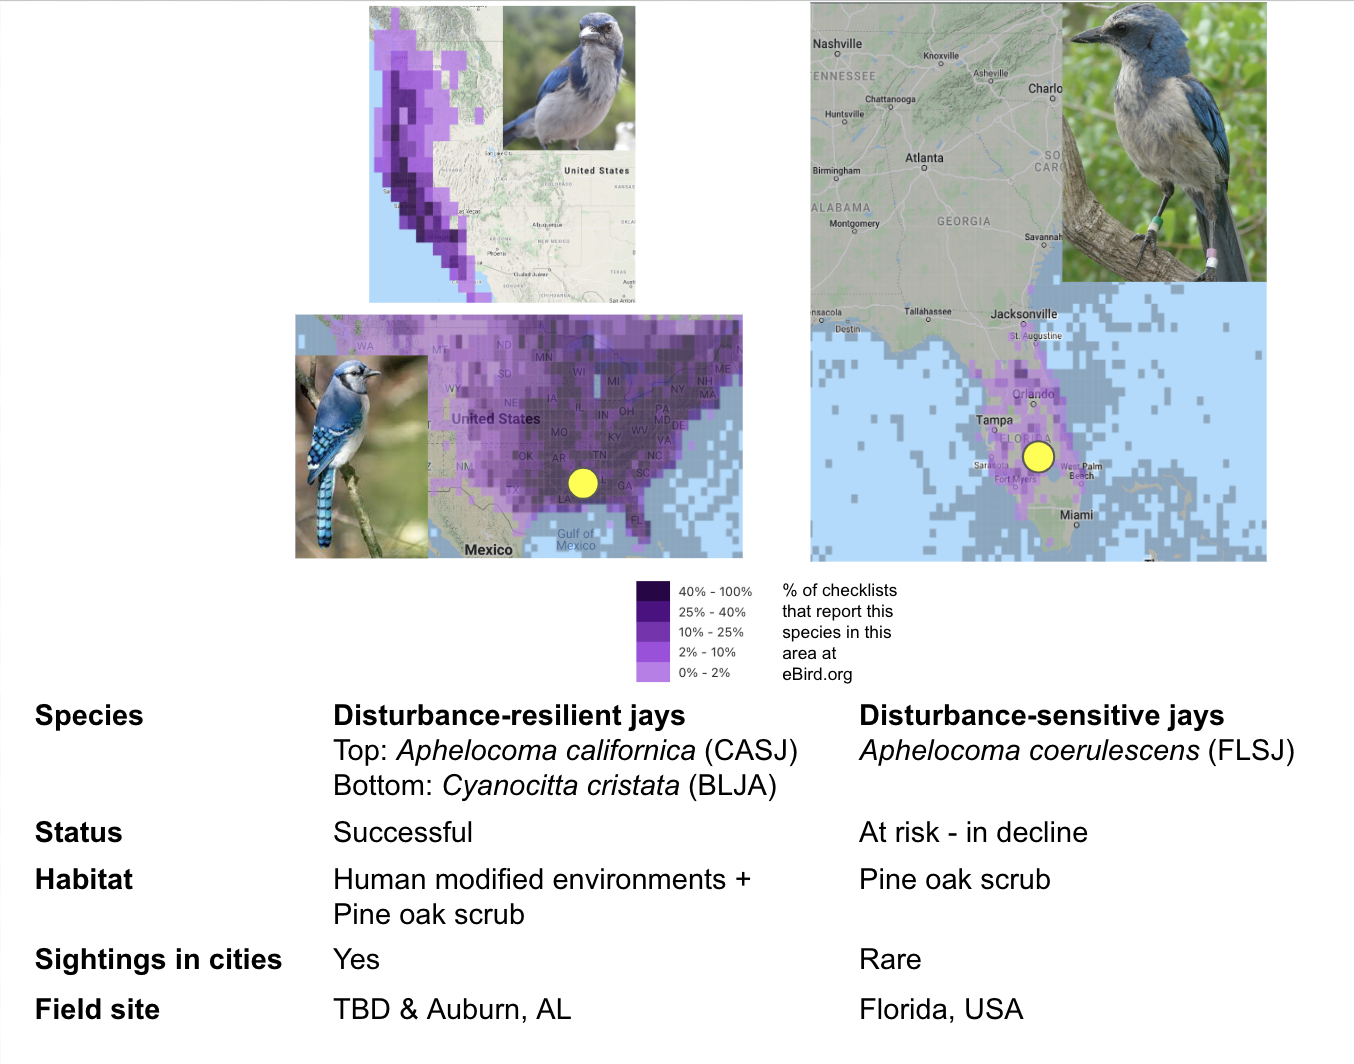
\includegraphics[width=1\linewidth,height=\textheight,keepaspectratio]{mi1jays_spp_Fig2.png}

\textbf{Figure 2.} Comparing the species involved in this investigation
relative to their geographic range and association with human modified
habitats. The yellow dots represent field site locations. Photo credit:
CASJ, Corina Logan; BLJA, Rhododendrites; FLSJ, VvAndromedavV.

~

\subsubsection{Background}\label{background}

Jay species exhibit a diversity of social systems and success in
colonizing suburban and urban areas (Fig. 2). California scrub-jays
(\emph{Aphelocoma californica}, hereafter ``CASJ'') and blue jays
(\emph{Cyanocitta cristata}, hereafter ``BLJA'') are singular,
monogamous breeders that are increasing in abundance, expanding their
range sizes, and highly successful in natural, suburban, and urban areas
(Blair, 1996; Curry et al., 2017). We therefore consider these
``disturbance-resilient'' (DR) jay species. In contrast, the Florida
scrub-jay (\emph{A. coerulescens}; hereafter ``FLSJ'') is a
``disturbance-sensitive'' (DS) jay species that is threatened, endemic,
and range-restricted to xeric oak scrub habitat in Florida (Woolfenden
\& Fitzpatrick, 1996).

These species forage primarily on mast (acorns, hazelnuts, etc.) that
they cache throughout their territory, which makes it available to eat
year-round. They are also opportunistic omnivores and specifically need
high-fat and high-protein arthropods to feed to nestlings and fledglings
(Curry et al., 2017). Nesting and foraging substrates can be drastically
different in human modified environments compared to natural areas
{[}e.g., predominance of non-native vegetation; Tuomainen \& Candolin
(2011){]}, and it is unknown whether suburban and urban jays are able to
persist in these environments through behavioral adjustments. The DS jay
species, the FLSJ, can persist in suburban habitats after conversion
from xeric oak scrub, however suburban populations of FLSJ steadily
decline (Bowman pers. comm.). This is potentially due to the presence of
suboptimal habitat resulting from fire suppression (Woolfenden \&
Fitzpatrick, 1996), higher rates of brood reduction through nestling
starvation (Shawkey et al., 2004), and the lack of nutritionally
complete prey items (Shawkey et al., 2004) in suburban habitats. It is
possible that behavioral flexibility in habitat use and foraging breadth
underlies the ability of some FLSJ to persist in human-dominated areas.

We aimed to compare behavioral flexibility within species, between
suburban and natural populations to determine whether variation in
flexibility relates to variation in presence in these habitats.
Subsequently, we planned to compare flexibility between DS and DR jay
species to determine whether this trait is related to the greater
success of DR jay species, like the CASJ and BLJA, in human-dominated
areas (but see Deviations section). Lastly, we tested whether
manipulating flexibility increases the foraging and microhabitat breadth
of jays in suburban and natural environments. Manipulating the
flexibility of a subset of individuals has the potential to affect the
population because previous research demonstrates that these species
have the capacity to use foraging information discovered by others
(social learning) to flexibly change their behavior (K. B. McCune et
al., 2022; Midford et al., 2000).

\subsubsection{Tailored Research
Questions}\label{tailored-research-questions}

For all research questions, Table 1 summarizes our predictions, analysis
plans, interpretations for the various directions the results could go,
and the hypotheses that could be contradicted given the various
outcomes.

\begin{itemize}
\tightlist
\item
  \textbf{J.Q1: Do jay populations in human modified areas differ in
  baseline behavioral flexibility compared to populations in natural
  areas?} We will investigate this question by comparing performance on
  serial reversal learning in the wild between jays in natural areas and
  jays in human modified areas.
\item
  \textbf{J.Q2: Are disturbance-resilient (DR) jays more behaviorally
  flexible than disturbance-sensitive (DS) jays?} We will investigate
  this question by comparing performance on serial reversal learning in
  the wild between DR and DS jay species.
\item
  \textbf{J.Q3: Does manipulating behavioral flexibility alter the
  number of microhabitats used?} We will investigate this question by
  tracking their presence in a variety of microhabitats before and after
  manipulating their flexibility using serial reversal learning in the
  wild. We only count that a microhabitat was used if the individual had
  at least 5\% of their data points there. This prevents a microhabitat
  from being counted even if an individual was simply moving through it,
  and therefore not necessarily using it.
\item
  \textbf{J.Q4: Does manipulating flexibility alter the number of
  different food items taken by jays?} We will investigate this question
  by tracking the various food items they take before and after
  manipulating their flexibility using serial reversal learning in the
  wild.
\end{itemize}

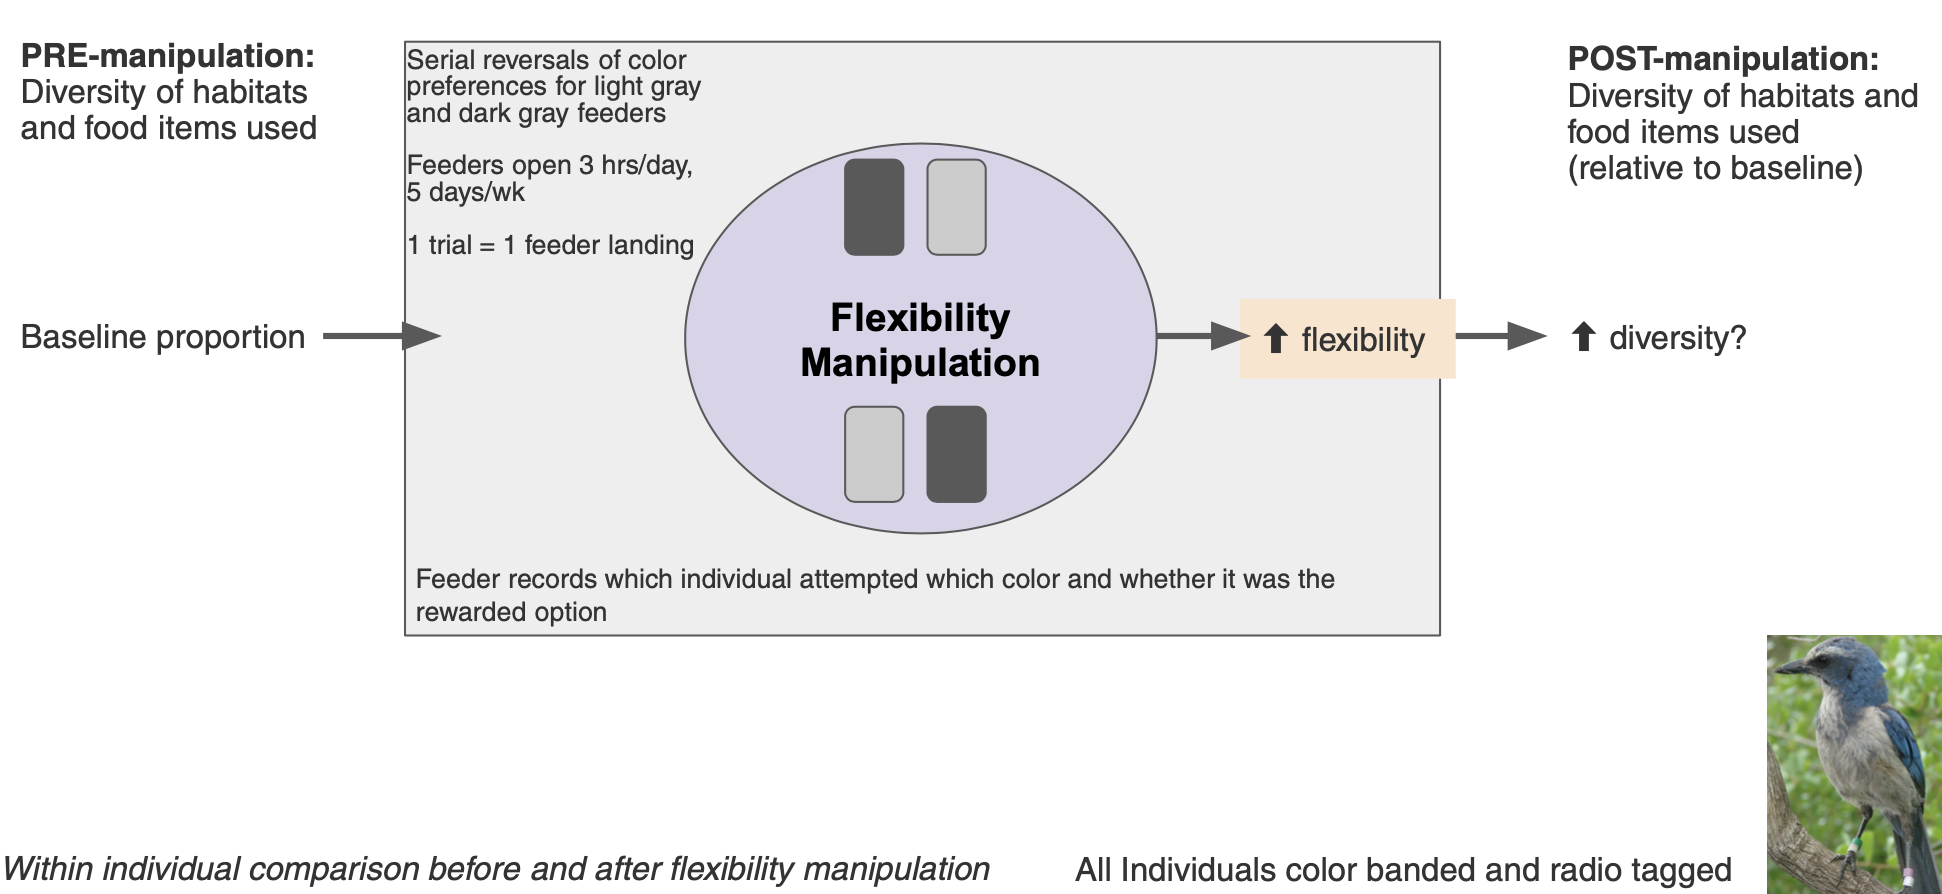
\includegraphics[width=0.8\linewidth,height=\textheight,keepaspectratio]{mi1Figjays.png}

\textbf{Figure 3.} The reversal learning experiment in a group context
(Design 2 from the ManyIndividuals registered report) tailored to the
jay research questions. The white rectangles represent feeder locations,
the feeder with the X is in the unrewarded location while the feeder
with the green check is the rewarded location.

\newpage

\textbf{Table 1.} Study design for the jay research. Note that we are
unable to test Q2 because it was not possible to sample CASJ or BLJA
within the timeframe of this study. References that were not already
cited in the introduction: Galbraith et al. (2015), Lapiedra et al.
(2017), Rice et al. (2003), Emery \& Clayton (2004), Sol et al. (2002),
Peterson et al. (2011), Grinnell (1917).
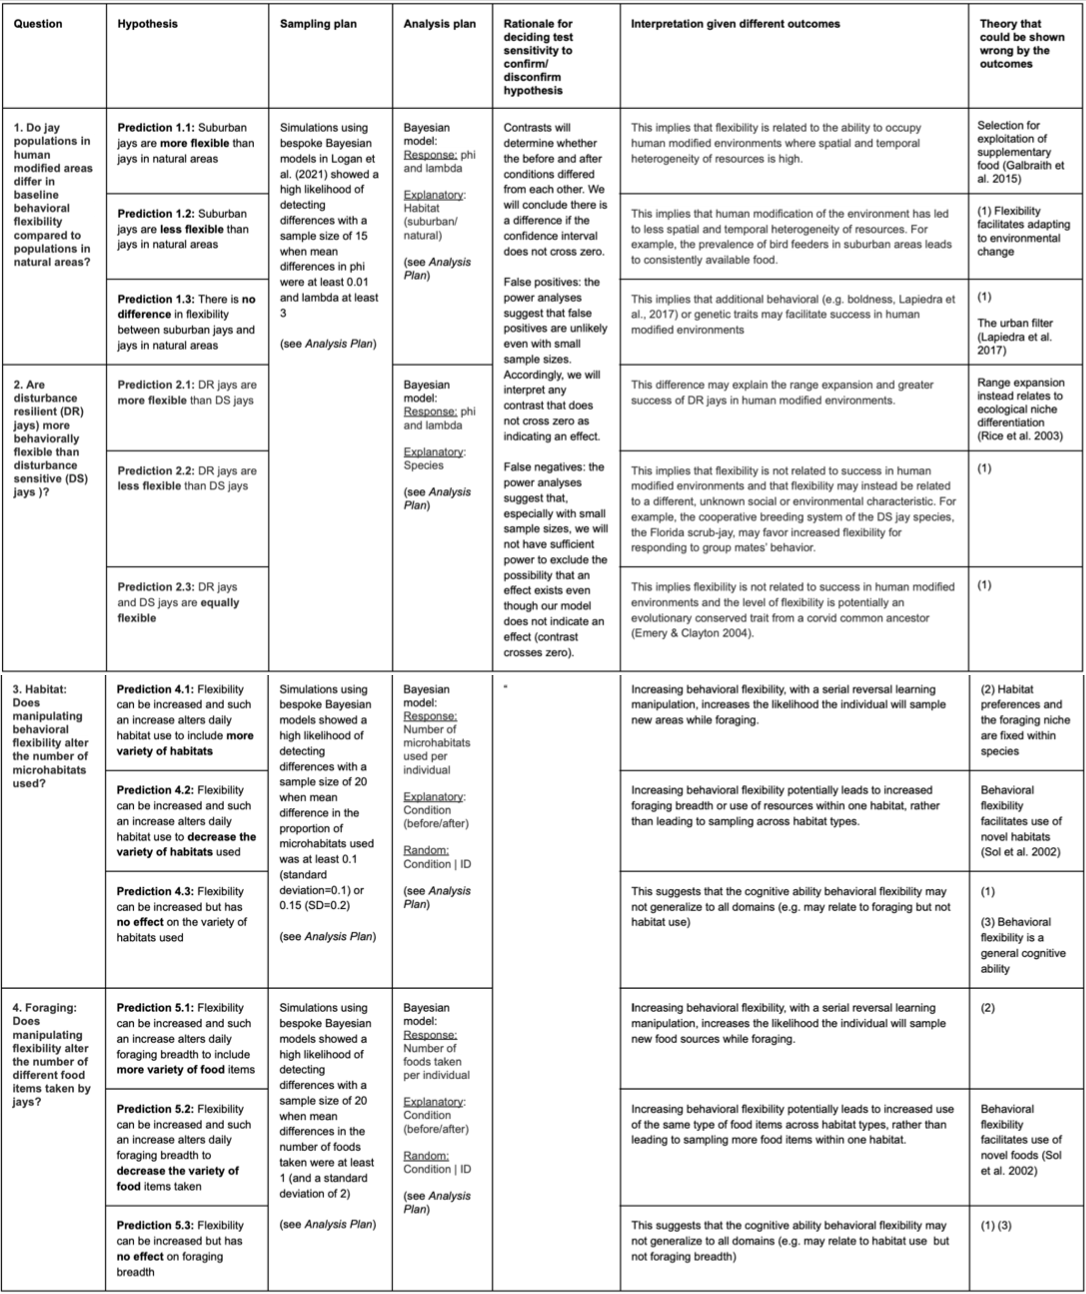
\includegraphics[width=1\linewidth,height=\textheight,keepaspectratio]{mi1StudyDesignTableJay.png}

\section{\texorpdfstring{\textbf{METHODS}}{METHODS}}\label{methods}

\subsection{Planned sample}\label{planned-sample}

We studied Florida scrub-jays in unfragmented, fire-maintained habitat
at Archbold Biological Station (natural areas), as well as in the
adjacent suburbs of Lake Placid, FL (human modified areas). Much of the
study population at Archbold Biological Station was already individually
identifiable with color leg bands. We caught an additional 24 jays using
walk-in traps and mist nets; collected their biometric data, and a blood
sample; applied colored leg bands; and released them at their point of
capture. We collected data on pre- and post-manipulation success
measures (foraging and habitat use, see below) and conducted the
experiment within the non-breeding season to control for potential
temporal differences in the environment and behavior. We planned to use
radio tags to find jays for observing before and after manipulation
success measures. However, Florida scrub-jays are highly territorial,
and we were always able to find the jays to collect observational data
without the radio tags.

To determine whether the flexibility manipulation has influenced the
ability of jays to persist in human modified environments, we planned
for half of the total sample of jays from areas with access to
human-supplemented food (i.e.~private property, university campus, parks
adjacent to neighborhoods with feeders) and the other half from natural
areas (wildlife management areas, reserves). To address Q1, testing for
differences in baseline behavioral flexibility between jays in natural
or human-modified environments, the power analysis (see Supplementary
materials S1) showed a high likelihood of detecting differences with a
minimum sample of 15. We were able to quantify baseline behavioral
flexibility in 14 Florida scrub-jays (8 in natural areas, 6 in
human-modified areas).

To address Q3 and Q4, we tracked baseline behavior and changes after the
flexibility manipulation via all-occurrence sampling during focal
observations (Altmann, 1974) that last for 60 min. During observations,
we documented all occurrences of microhabitats used within the territory
and foraging behavior (see Observational methods, below). Our planned
minimum sample size was 20 individuals per species with a minimum of 4
observations per individual (at least 2 per month) pre-manipulation and
a minimum of 4 per individual (at least 2 per month) post-manipulation
(at least 320 observations in total). We were only able to conduct the
serial reversal manipulation on 9 color-banded individuals, but we met
or exceeded the minimum sample size for observations before and after
the manipulation. There was one exception where an individual
disappeared after the manipulation and was not found during extensive
searching of the territory and surrounding areas and so was presumed
dead. We only collected one-third of the necessary post-manipulation
data on this individual.

\subsection{Observational methods}\label{observational-methods}

During observations, we recorded each microhabitat the individual is
present in and all food items consumed. Before data analysis, to ensure
that we were only including the microhabitats individuals use (rather
than just pass through), we filtered the data to include only
microhabitats that account for at least 5\% of their data points.
Although we may not observe every possible microhabitat or food item the
individual may use, by equally sampling before and after the
manipulation we can detect changes in habitat use. We counterbalanced
observations across the morning and afternoon for all individuals in the
study. In this way, we collected a random sample of data from active and
inactive time periods for all individuals.

Microhabitat types in the suburban habitat (\textless100m from human
structure) included: vertical human structure (e.g.~building, bench),
native vegetation, non-native vegetation, grass, impervious surface, and
dirt. In the natural habitat (\textgreater100m from human structure),
microhabitat types included all previous categories, but not human
structure or impervious surface. All categories were further defined by
whether the subject was high (\textgreater3m) or low (\textless3m). For
example, grass and impervious surfaces can occur above 3m if grass is on
the roof of a building, and if an individual is walking on the
impervious surface of an upper floor parking garage.

Food types were broken down into plant (seed, fruit, human-provided, or
unknown plant) and animal (insect larva, adult insect, amphibian,
crustacean, reptile, mammal, bird, egg, human-provided, or unknown
animal). ``Human-provided'' indicates any food item that was acquired
from a store at some point and is left out by humans. For example,
sunflower seeds would be considered human-provided if they are in the
form of bird seed or a human snack. Sunflower seeds would only be
counted in the ``seed'' category if the bird is seen eating it from a
plant.

Additionally, for all observations we used binoculars so that we could
remain far enough from the focal individual that our presence was not
affecting their behavior. Because that distance can be different for
each individual and species, we hesitate to give a specific number.
However, if at any point the focal individual showed that it was
affected by our presence, by looking directly at the researcher, alarm
calling or startling, then we ended the observation immediately, dropped
all data from that observation session and attempted the observation
again the next day.

\subsection{Flexibility manipulation (Design 2 from the registered
report)}\label{flexibility-manipulation-design-2-from-the-registered-report}

Our approach involved individual jays participating in a serial reversal
learning task in the wild. We set up remote-controlled feeders at
multiple study sites, each containing several jay territories, spaced at
least 2km apart: 2 sites in natural habitat, 2 in human-modified
habitat.

\subsubsection{Feeder habituation}\label{feeder-habituation}

One feeder at each location contained food and the experimenter used the
remote to feed the focal individual every time it approached.
Habituation consisted of 2-hour sessions between 8a-3p on a minimum of 4
consecutive days or until at least 1 banded jay per territory had
visited the feeder at least 3 times without showing fear behaviors.

\subsubsection{The experiment}\label{the-experiment}

Prior to the flexibility manipulation, we collected the 4 minimum
observation sessions to determine the baseline values for microhabitat
use and foraging breadth. Afterwards, we set up the remote-controlled
feeders to initiate the serial reversal learning flexibility
manipulation phase. All feeders contained one type of high value food
(i.e., peanuts). In addition, feeders were opaque and always had food in
them to eliminate a confound with performance due to olfactory
differences between the feeders that could be introduced if only the
rewarded feeders had food in them. If a feeder needed to be refilled, we
refilled all feeders consecutively in the same time period and for the
same amount of time even if that feeder did not need much or any food
(in these cases, we pretended to fill the feeder). This eliminated
potential confounds in jay performance from cues provided by a
differential amount of experimenter attention given to the feeders
during refilling.

At the beginning of serial reversal learning, one of the two feeders, at
a consistent location (north or south, east or west) within the
territory, was randomly selected to dispense food when the focal jay
approached. If the subject visited the non-rewarded feeder, this
incorrect choice was recorded, but the feeder did not open. Reversal
sessions for the manipulation treatment consisted of 30-120 min sessions
per day per territory, up to 4 days per week. Each visit by the focal
jay to the correct or incorrect feeder was considered a trial. Jays
passed a given reversal when they correctly chose the rewarded feeder in
at least 10 trials out of the most recent 12 trials (see S1 of the
supplementary materials for details on the simulations that determined
that threshold). After passing one reversal, we switched to rewarding
jays at the other feeder location. Serial reversals continued until jays
passed two consecutive reversals in 12 trials or less (see S2 of the
supplementary materials for details on the simulations that determined
that threshold). At this criterion, the jays were considered to have
increased their behavioral flexibility.

After the manipulation was complete for the focal individual, we again
conducted the all-occurrences focal observation sessions to measure
microhabitat use and foraging breadth. We began collecting
post-manipulation data on an individual as soon as it passed the
manipulation because it is unknown for how long any potential effects of
the manipulation will last.

For more social species, like the Florida scrub-jay, who may experience
the experiment in groups, there is the potential that individuals who
were not in the manipulation condition or who have not yet passed the
manipulation condition will learn about post-manipulation success
behaviors from the manipulated individuals who passed the experiment. We
are ultimately interested in determining whether we can change success
behaviors of threatened populations or species as a result of the
flexibility manipulation. If part of this change is the result of social
learning from some of the manipulated individuals, it will still result
in a change even if we do not quantify what percentage of the mechanism
comes from individual learning as a result of the manipulation or social
learning after the manipulation. If there is a change in success
measures between before and after the manipulation, the manipulation
will have been the cause in either case.

\subsection{Open data}\label{open-data}

The data will be published in the Knowledge Network for Biocomplexity's
data repository.

\subsection{Protocols}\label{protocols}

\begin{itemize}
\tightlist
\item
  Jay
  \href{https://docs.google.com/document/d/1VWL7AIDB-Z1vhs1dEM7JACHuvNjgjZCBI3ubQECqm2U/edit?usp=sharing}{protocol}
  and
  \href{https://docs.google.com/spreadsheets/d/1qpukS67A8IslPxP8RBpdB4fS4f9ofWCvQXVgXu-G7Qs/edit?usp=sharing}{data
  sheet templates}
\item
  \href{https://docs.google.com/document/d/1ZOpkdxy5-wiGg7hYod-XaaBoOl53DsVQ3pwWoIdvrzk/edit?usp=sharing}{Protocol
  for applying radio tags and conducting GPS tracks} from McCune KB et
  al. (2020)
\item
  Jay
  \href{https://docs.google.com/document/d/1YnGdsU-Q7kNBVT-N3x1BA30xP10jPFYEv9-dlTw2RcQ/edit?usp=sharing}{processing
  protocol}
\end{itemize}

\subsection{Analysis plan}\label{analysis-plan}

We run analyses in R {[}current version 4.5.0; R Core Team (2017){]}
using the following R packages: rethinking (McElreath, 2020a), rstan
(Stan Development Team, 2020), cmdstanr (Gabry \& Češnovar, 2022), knitr
(Xie, 2018), and irr (Gamer et al., 2012). We describe below the
Bayesian models we developed to address each of the specific research
questions. All Bayesian models were developed using McElreath (2020b) as
a guide. Code for running these models is available in supplementary
materials S4.

\subsubsection{J.Q1 Do jay populations in human modified areas differ in
baseline behavioral flexibility compared to populations in natural
areas?}\label{j.q1-do-jay-populations-in-human-modified-areas-differ-in-baseline-behavioral-flexibility-compared-to-populations-in-natural-areas}

\textbf{The model}

We used the reversal learning Bayesian model in Logan CJ et al. (2020)
to simulate and analyze population differences in reversal learning, and
calculate our ability to detect differences between populations. The
model ``accounts for every choice made in the reversal learning
experiment and updates the probability of choosing either option after
the choice was made depending on whether that choice contained a food
reward or not. It does this by updating three main components for each
choice: an attraction score, a learning rate (\(\phi\)), and a rate of
deviating from learned attractions (\(\lambda\))'' (Logan CJ et al.,
2020).

\textbf{\emph{Equation 1 (attraction and \(\phi\)):}}
\(A_{i,j, t+1} = (1-\phi_j) A_{i,j,t} + \phi_j \pi_{i,j,t}\)

Equation 1 ``tells us how attractions to different behavioral options
\(A_{i,j, t+1}\) (i.e., how preferable option \(i\) is to the bird \(j\)
at time \(t+1\)) change over time as a function of previous attractions
\(A_{i ,j, t}\) and recently experienced payoffs \(\pi_{i,j,t}\) (i.e.,
whether they received a reward in a given trial or not). Attraction
scores thus reflect the accumulated learning history up to this point.
The (bird-specific) parameter \(\phi_j\) describes the weight of recent
experience. The higher the value of \(\phi_j\), the faster the bird
updates their attraction. It thus can be interpreted as the
\emph{learning or updating rate of an individual}. A value of
\(\phi_j = 0.04\), for example, means that receiving a single reward for
one of the two options will shift preferences by 0.02 from initial
0.5-0.5 attractions, a value of \(\phi_j = 0.06\) will shift preferences
by 0.03 and so on'' (Blaisdell et al., 2021).

\textbf{\emph{Equation 2 (\(\lambda\)):}}
\(P(i)_{t+1} = \frac{\exp(\lambda_j A_{i, j, t})}{\sum\limits_{m=1}^{2}\exp(\lambda_j A_{m, j, t})}.\)

Equation 2 ``expresses the probability an individual \(j\) chooses
option \(i\) in the next round, \(t+1\), based on the latent
attractions. The parameter \(\lambda_j\) represents the \emph{rate of
deviating from learned attractions} of an individual (also called
inverse temperature). It controls how sensitive choices are to
differences in attraction scores. As \(\lambda_j\) gets larger, choices
become more deterministic, as it gets smaller, choices become more
exploratory (random choice if \(\lambda_j = 0\)). For instance, if an
individual has a 0.6-0.4 preference for option A, a value of
\(\lambda_j = 3\) means they choose A 65\% of the time, a value of
\(\lambda_j = 10\) means they choose A 88\% of the time and a value of
\(\lambda_j = 0.5\) means they choose A only 53\% of the time''
(Blaisdell et al., 2021).

We used the c values as the response variable in the Bayesian model to
examine whether there were differences in flexibility between the
habitats:

y \textasciitilde{} \(\alpha\){[}habitat{]}

y is the response variable (\(\phi_j\) and \(\lambda_j\), which are
extracted from the correct and incorrect choices in the serial
reversals). There is one intercept, \(\alpha\), per habitat (suburban or
natural) and we will estimate the habitat's average and standard
deviation of the response variable.

\subsubsection{J.Q2 Are disturbance-resiliant jays more flexible than
disturbance-resistant
jays?}\label{j.q2-are-disturbance-resiliant-jays-more-flexible-than-disturbance-resistant-jays}

We were not able to collect data on disturbance-resilient species within
the timeframe of this study and the funding of our grant. However, we
were able to conduct an \emph{unregistered analysis} testing for
differences in behavior between disturbance-resilient Florida scrub-jay
individuals persisting in human-modified areas and conspecifics in
natural habitat lacking human disturbance.

\textbf{The model}

We used poisson regression to assess whether jays in human-modified
areas foraged on more kinds of foods and used more substrate types
relative to jays in natural areas. Models were not overdispersed or
heteroscedastic.

\subsubsection{J.Q3 More flexible = use more
microhabitats?}\label{j.q3-more-flexible-use-more-microhabitats}

\textbf{The model}

\emph{Bayesian model with a normal distribution:}

habitatuse \textasciitilde{} \(\alpha\){[}ind{]} +
\(\beta\){[}ind{]}*before

habitatuse is the response variable: the total number of different
microhabitats used per individual. There was one intercept, \(\alpha\),
and one slope \(\beta\) per individual, which was estimated for the two
conditions, before (and after) the manipulation. ID is nested within
condition as a random effect because there was more than one data point
per individual: each individual has a data point in the before condition
and in the after condition. A normal distribution was used because the
response variable is a sum without an expected skew to the curve (see
Figure 10.6 in McElreath, 2020b).

\subsubsection{J.Q4 More flexible = more food
types?}\label{j.q4-more-flexible-more-food-types}

\textbf{The model}

\emph{Bayesian model with a normal distribution:}

y \textasciitilde{} \(\alpha\){[}ind{]} + \(\beta\){[}ind{]}*before

y is the response variable: the total number of different food types
taken per individual. There will be one intercept, \(\alpha\), and one
slope \(\beta\) per individual, which will be estimated for the two
conditions, before (and after) the manipulation. ID is nested within
condition as a random effect because there is more than one data point
per individual: each individual has a data point in the before condition
and in the after condition. A normal distribution was used because the
response variable is a sum without an expected skew to the curve (see
Figure 10.6 in McElreath, 2020b).

\section{\texorpdfstring{\textbf{RESULTS}}{RESULTS}}\label{results}

Very few Florida scrub-jay were found in human-modified areas at our
study site in Lake Placid, FL. Across two years we collected focal
observations and baseline behavioral flexibility on 6 individuals in
these human-modified areas and 8 jays in natural areas at Archbold
Biological Station. A smaller subset of 9 jays (all 8 jays in the areas
and 1 from the human-modified areas) received the serial research
learning flexibility manipulation because it was not feasible to conduct
this longer experiment on more jays within the constraints of our field
season.

\subsection{J.Q1 Do jay populations in human modified areas differ in
baseline behavioral flexibility compared to populations in natural
areas?}\label{j.q1-do-jay-populations-in-human-modified-areas-differ-in-baseline-behavioral-flexibility-compared-to-populations-in-natural-areas-1}

There was no difference in baseline behavioral flexibility performance
between jays in suburban or natural areas. This was true when we
considered either of the two behavioral flexibility components,
\(\phi_j\), the rate of learning the newly rewarded option (\(\beta\) =
-0.23, sd = 1.27, CI = -2.22 - 1.4, \emph{p} \textgreater{} 0.05), or
\(\lambda_j\), the rate of deviation from previously rewarded options
(\(\beta\) = -0.01, sd = 0.18, CI = -0.28 - 0.28, \emph{p}
\textgreater{} 0.05).

\pandocbounded{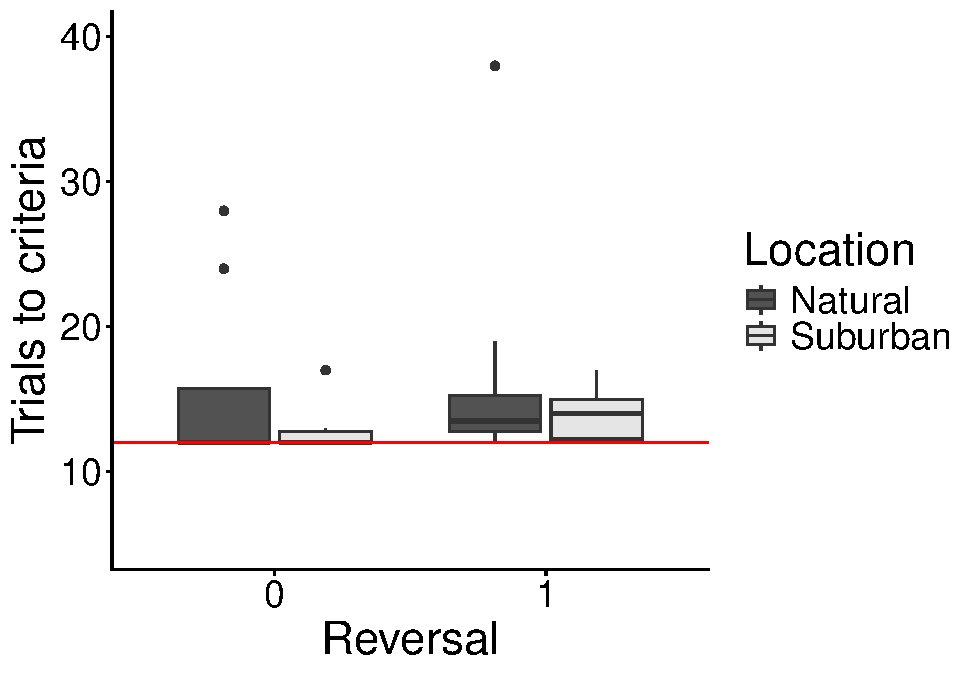
\includegraphics[keepaspectratio]{mi1jays_files/figure-latex/plotjayflexbefore-1.pdf}}
Figure 3: Before the flexibility training, jays in the suburban and
natural habitats performed exceptionally well on the baseline behavioral
flexibility task and did not differ in ability. These boxplots show the
performance as the number of trials to reach the passing criterion on
baseline associative learning (Reversal 0) and behavioral flexibility
(Reversal 1) for jays in the natural (dark grey) and human modified
(light grey) areas. We use trials to pass, rather than or in this plot
for more interpretable illustration of the speed of performance on this
task. The horizontal red line illustrates the minimum number of trials
to pass criteria (10 out of the most recent 12 trials correct).

\subsection{J.Q2 Are disturbance-resilient jays more flexible than
disturbance-resistant
jays?}\label{j.q2-are-disturbance-resilient-jays-more-flexible-than-disturbance-resistant-jays}

We were not able to test this question within the timeframe and funding
of the grant. However, we conducted an unregistered analysis using
Poisson models to compare foraging and habitat use behavior of Florida
scrub-jays in human modified areas to those in natural areas. In other
words, within this disturbance sensitive species, a subset of
individuals were resilient to disturbance, at least during the timeline
of this study. The disturbance-resilient individuals in the suburbs were
not more diverse foragers (\(\beta\) = 0.26 ± 0.19, \emph{p} = 0.15),
but did use a greater variety of microhabitats (\(\beta\) = 0.52 ± 0.16,
\emph{p} = 0.001) compared to the jays in undisturbed, natural habitat
at Archbold Biological Station.

\subsection{J.Q3 More flexible = use more
microhabitats?}\label{j.q3-more-flexible-use-more-microhabitats-1}

Even though all jays increased the speed with which they switched their
preference in the serial reversal learning training, there was no effect
on subsequent habitat use diversity (before relative to after log-odds
difference = -0.06, CI = -0.41 - 0.30, \emph{p} \textgreater{} 0.05;
Fig. 4).

\subsection{J.Q4 More flexible = more food
types?}\label{j.q4-more-flexible-more-food-types-1}

Similarly, after the serial reversal flexibility training, jays were not
more likely to eat a greater diversity of food types (\(\beta\) = 0.26,
CI = -0.45 - 0.96, \emph{p} \textgreater{} 0.05; Fig. 4).

\pandocbounded{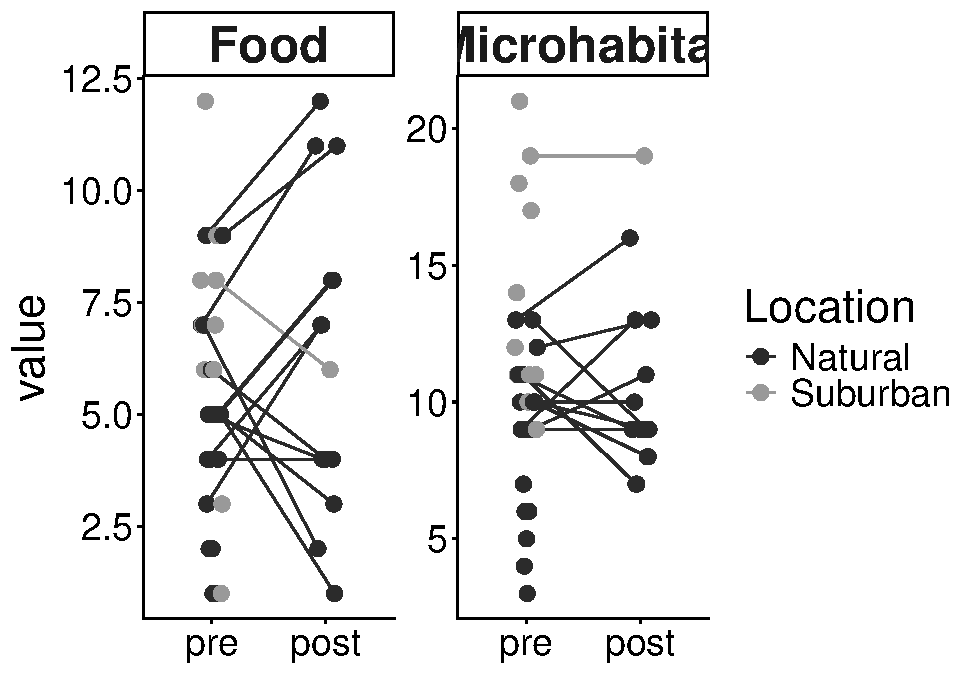
\includegraphics[keepaspectratio]{mi1jays_files/figure-latex/plotfor-habitatuse-1.pdf}}
Figure 4: Jays did not predictably change their foraging or microhabitat
use behaviors after they underwent the flexibility training
manipulation. Values indicate the number of different foods or
substrates jays were observed to use during the all-occurrences focal
observation session before (pre) and after (post) we conducted serial
reversal learning to increase behavioral flexibility. Each dot
represents a jay and lines connect the dots of jays with data both pre
and post. We collected pre observations on some jays for which we were
not able to conduct the flexibility training and so we did not need to
collect post observations.

\section{\texorpdfstring{\textbf{DISCUSSION}}{DISCUSSION}}\label{discussion}

Anthropogenic change is creating unpredictable heterogeneity in the
environment that requires some level of fast, adaptable learning in
wildlife populations. In some species, the general cognitive trait,
behavioral flexibility, is thought to underlie the ability to cope with
rapid changes in human-modified environments (Sol et al., 2002; Vardi \&
Berger-Tal, 2022). Our previous work in the great-tailed grackle
supported this hypothesis because grackles that were trained to be more
flexible foraged on more diverse food and used more distinct behaviors
to forage in the wild (Logan et al., 2025). The grackle is an
urban-adapted generalist species that has demonstrated adaptability to
environmental change through a rapid range expansion (Wehtje, 2003). We
tested whether the same training to increase behavioral flexibility in a
threatened species, the Florida scrub-jay (FLSJ), would lead to more
adaptable foraging and habitat use behaviors in the wild. However, we
found no effect of the behavioral flexibility training in this species.

Unlike great-tailed grackles, FLSJ populations have rapidly declined
coincident with anthropogenic change and there is little evidence for
adaptation to human-modified environments. Yet, for many species,
suburban environments can also provide significantly more foraging
opportunities through the provision of novel foods, ornamental plants or
agricultural activities that increase survival and reproductive success.
For example, use of food at bird feeders has been linked to population
growth and range expansions (Greig et al., 2017; Veech et al., 2011).
One such species is the California scrub-jay, a congener to the FLSJ,
that similarly prefers xeric scrub-oak habitat along the west coast of
the United States. In contrast to the FLSJ, this species has been able
to adapt to persist in highly developed areas (e.g., Los Angeles, CA)
and expand its range north, while taking advantage of bird feeders
(Curry et al., 2017).

In our population of FLSJ, a small population does persist in suburban
areas. Anecdotally, homeowners report frequently seeing these
individuals at their backyard bird feeders or other human-provided food
sources. We compared foraging and habitat use of these individuals to
FLSJ in pristine, unfragmented and fire-maintained scrub habitat at
Archbold Biological Station. Jays in both habitat types foraged on
equally diverse food items, but suburban jays used more distinct kinds
of microhabitats (substrate type and height) relative to the jays at
Archbold. In other words, suburban jays did not completely restrict
their habitat use to the small remnant fragments of undeveloped scrub in
the suburbs. This demonstrates that FLSJ are capable of adapting their
habitat use behavior to include novel, human-modified environments.
However, when we compared baseline behavioral flexibility between the
two jay populations, suburban jays were not more behaviorally flexible
than Archbold jays. Consequently, it is likely that behavioral
flexibility, as we measured it through spatial reversal learning, does
not underlie adaptation to human-disturbance in this species.

This was supported by our finding of no change in foraging and habitat
use behavior after undergoing behavioral flexibility training. Our
results support our Prediction 1 alternative 1; all jays improved their
reversal learning speed to meet the criterion, indicating they had
increased their behavioral flexibility. But there was no consistent
trend in the change in food item or microhabitat diversity measured
before and after the training. There are a few potential explanations
for why the training worked in great-tailed grackles but led to no
behavior change in FLSJ. First, it is possible that the serial reversal
learning task and passing criterion were too easy for FLSJ and so the
training did not lead to a large enough change in flexibility to be seen
in resulting behavior. We based the criteria for when an individual was
considered to have passed a given reversal, as well as for passing the
whole flexibility training, on performance of great-tailed grackles in
the previous, similar experiment. However, FLSJ were significantly
faster at forming an initial understanding of the location of the
rewarded feeder and subsequently reversing that association compared to
the grackles. In fact, the majority of individuals achieved the passing
criteria almost as quickly as possible (Fig. 3). Our criterion to pass
was 10 correct choices out of the most recent 12 trials and half of the
jays reached this criterion in 12 or 13 trials (average = 15.6, max =
38). In comparison, the average number of trials for great-tailed
grackles to reach criterion in the first reversal was 75 (K. McCune et
al., 2023). This drastic difference in performance could be because
grackles were tested in captivity and jays were tested in the wild (K.
B. McCune et al., 2019). Although, another study (Bebus et al., 2016)
evaluated reversal learning of FLSJ in captivity and those individuals
required a similar number of days (3 days) to pass the criterion as in
our study (2.8 days), but it is unclear if grackles would perform better
if tested in the wild.

Another potential reason we failed to see a change in natural behavior
after the flexibility training is that jays were already using the
majority of foods and substrates available. Due to time constraints,
size and accessibility of the suburban population, the majority of jays
(8 out of 9 total) that underwent the flexibility training were from
Archbold Biological Station where the scrub-oak habitat is maintained at
high quality and mid-successional state through prescribed fire and
other management techniques. Thus, this habitat is far more homogenous
than jays experience in the suburban areas. Consequently, it is possible
that there was no opportunity for flexibility training to alter the
foods or microhabitats used by these jays. However, this is unlikely to
be a large confound because the suburban and Archbold jays did not
differ in the number of different food items they ate before training
and the one jay from the suburban area that we were able to train, also
did not show a change in the variety of substrates used and showed a
slight decrease in the diversity of food items used after the training
(Fig. 4, single grey line).

To better understand the role of behavior in adaptation or resilience to
human disturbance, ongoing and future work in FLSJ will evaluate
variation in other relevant behavioral traits like boldness, foraging
role (producer-scrounger dynamics), exploration and movement behavior
(Snell-Rood \& Steck, 2019). The ManyIndividuals registered report also
creates a versatile structure for testing behavioral flexibility in
other species or systems. Although we were unable to test disturbance
resilient jay species within the timeline of our current funding, we
hope the research we present here will provide guidance and motivation
for other investigators to address this question. As humans accelerate
the frequency and degree of environmental change, experimental
interventions such as this, that train species in behaviors that
facilitate resilience, may become increasingly important.

\section{\texorpdfstring{\textbf{ETHICS}}{ETHICS}}\label{ethics}

This research is carried out in accordance with permits from the:
\textbf{1.} US Fish and Wildlife Service (scientific collecting permit
number ES824723). \textbf{2.} US Geological Survey Bird Banding
Laboratory (federal bird banding permit number 07732). \textbf{3.}
Institutional Animal Care and Use Committee (University of California
Santa Barbara protocol number 958 and Auburn University protocol number
2022-5132).

\section{\texorpdfstring{\textbf{AUTHOR
CONTRIBUTIONS}}{AUTHOR CONTRIBUTIONS}}\label{author-contributions}

\textbf{McCune:} Hypothesis development, data collection, data analysis
and interpretation, write up, revising/editing.

\textbf{Barve:} Interpretation, revising/editing, materials/funding

\section{\texorpdfstring{\textbf{FUNDING}}{FUNDING}}\label{funding}

This research is funded by the Department of Human Behavior, Ecology and
Culture at the Max Planck Institute for Evolutionary Anthropology (to
Logan and McCune).

\section{\texorpdfstring{\textbf{CONFLICT OF INTEREST
DISCLOSURE}}{CONFLICT OF INTEREST DISCLOSURE}}\label{conflict-of-interest-disclosure}

We, the authors, declare that we have no financial conflicts of interest
with the content of this article.

\section{\texorpdfstring{\textbf{ACKNOWLEDGEMENTS}}{ACKNOWLEDGEMENTS}}\label{acknowledgements}

We are grateful to our funders: Richard McElreath at the Max Planck
Institute for Evolutionary Anthropology (whole project), as well as
Corina Logan and Dieter Lukas for assistance with analyses and coding.
In addition, we are grateful for the ManyIndividuals co-founders, Drs.
Corina Logan and Rachel Shaw. We are thankful for the input and
assistance of Dr.~Reed Bowman when designing the Florida scrub-jay data
collection.

\section{\texorpdfstring{\textbf{SUPPLEMENTARY
MATERIALS}}{SUPPLEMENTARY MATERIALS}}\label{supplementary-materials}

\subsection{S1 - Determining when to switch each individual to the next
reversal: reversal passing
criterion}\label{s1---determining-when-to-switch-each-individual-to-the-next-reversal-reversal-passing-criterion}

Different criteria exist to decide whether an individual has learned an
association between the presence of a reward and some other feature
(e.g., color or shape). The two main two criteria used are to switch an
individual after it either has chosen 10 out of 12 choices correct
(e.g., Shaw et al., 2015) or 17 out of 20 choices correct (e.g., C. J.
Logan, 2016). The criteria are further modified depending on whether
choices are assessed continuously or grouped in predetermined blocks.

Here, we assess whether achieving 10 correct choices out of the last 12
continuously counted choices can be used as a reliable reversal passing
criterion. To determine reliability and suitability, we investigated
five questions (see below) by generalizing previously simulated reversal
learning data from Logan CJ et al. (2020), based on data from
great-tailed grackles. We simulated the choices individuals with
different learning rates (phi) and rates of deviating from learned
associations (lambda) would make in the initial discrimination and in
the first reversal. Grackles are fast to reverse preferences compared
with many other species (C. J. Logan, 2016), therefore we generalized
the simulations to other species by setting the parameters that guide
performance (phi and lambda) to lead to slower performances.

The findings from these simulated data indicate that deciding that an
individual has passed the reversal when they choose 10 out of the last
12 consecutive trials correctly is functional and reliable because of
the following:

\textbf{1) individuals will be finished after fewer trials than with
other criteria}

With the 10 out of 12 criterion, individuals pass the reversal 8 trials
faster (median) than with the 17 out of 20 criterion. This means that,
for most individuals, the two rules are equally effective because they
will pass both in the same amount of trials (i.e., the individual who
met the 17/20 criterion in 50 trials would have met the 10/12 criterion
in 42 trials), but because the 10 out of 12 criterion is restricted to
12 trials instead of 20, individuals need 8 fewer trials to meet the
passing criterion. No individual needs more trials with the 10 out of 12
criterion. When trials are grouped into blocks of 10 such that they
could only pass on trial 20, 30, etc., individuals need a median of 5
more trials compared to when choices are assessed continuously.

\textbf{2) classification of individuals using the 10/12 criterion is
less noisy because there is less of a chance for individuals to approach
the criterion and not pass or never pass}

The average improvement in the number of trials individuals need to
reach the respective criterion is larger than the median of 8 trials.
This occurs because there are no individuals who are faster with the 17
out of 20 criterion, and because there is a subset of individuals who
need considerably fewer trials with the 10/12 criterion (Figure 7).
Individuals who require a larger number of trials (\textgreater100) to
pass almost never occur with the 10/12 criterion, whereas they are more
common with the 17/20. With more trials, there is a higher chance that
an individual will deviate from their preference by chance. This is also
reflected in that 65 of the 626 simulated individuals never reached the
17/20 criterion within the maximum 300 trials, whereas there were only 4
individuals with the 10/12 criterion. Accordingly, an additional benefit
of choosing the 10/12 criterion is that it is more likely that data for
all individuals, even those who are slow to learn an association, can be
collected.

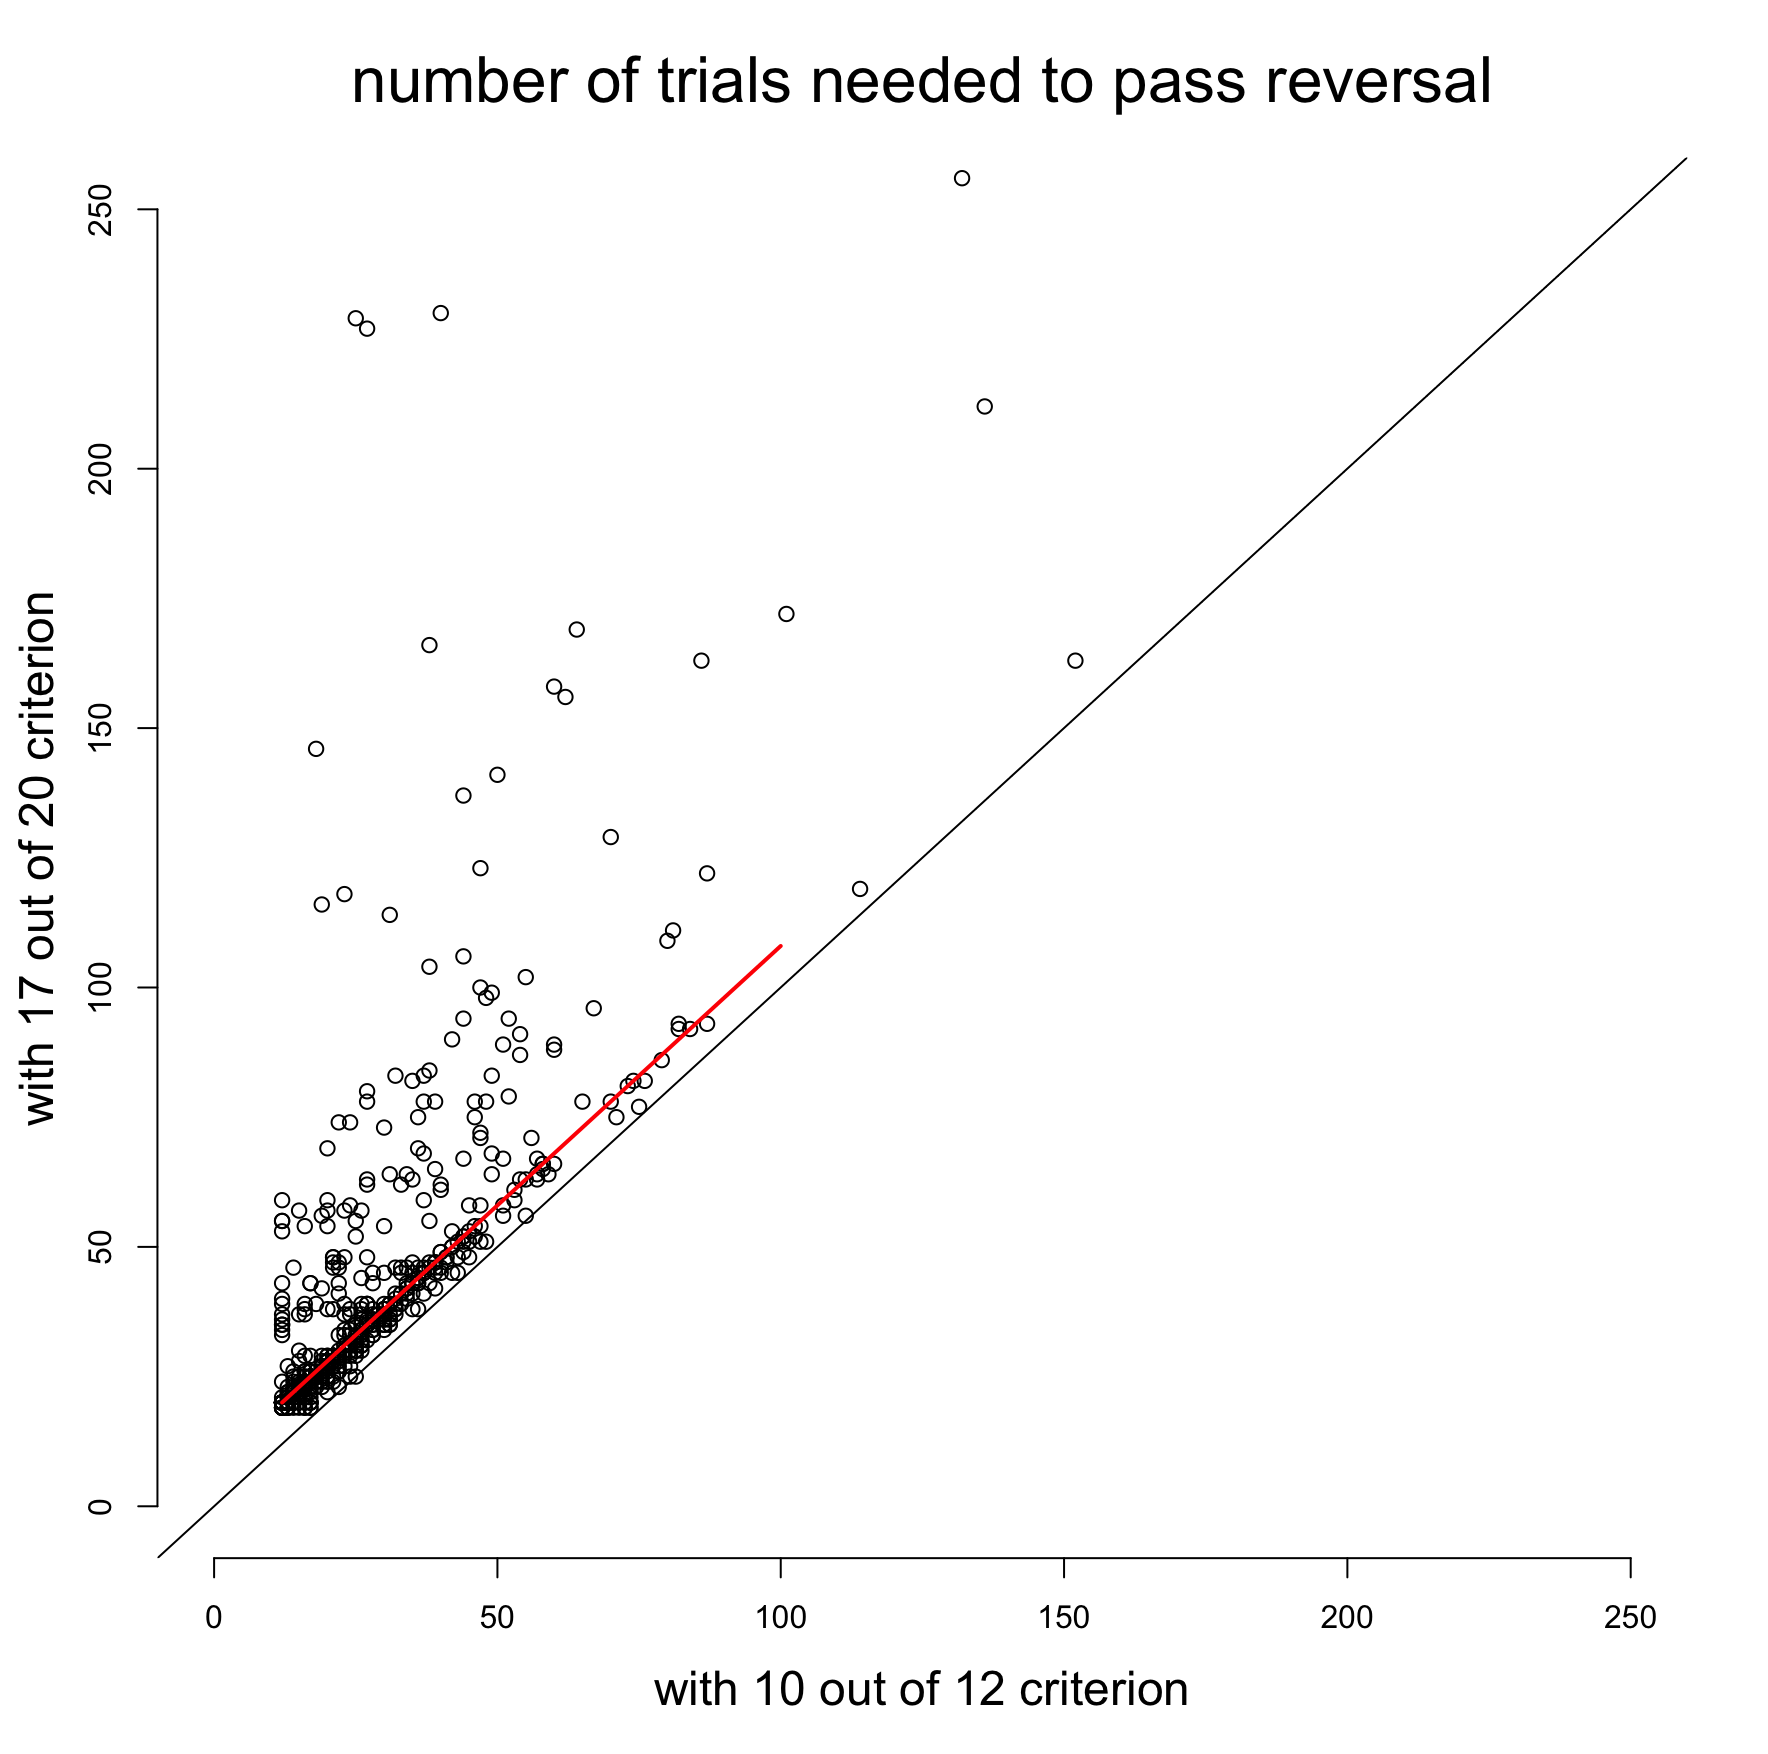
\includegraphics[width=0.6\linewidth,height=\textheight,keepaspectratio]{m1Fig_ReversalCriterionComparison.png}

\textbf{Figure S1.} There is less variation with the 10/12 reversal
learning passing criterion and it requires fewer trials to reach than
the 17/20 passing criterion. The lines represent the densities of
individuals (estimated with smoothing which means values can go down to
zero) across the 626 simulated individuals that needed a certain number
of trials to either reach the 10/12 (red) or the 17/20 (black)
criterion. With the 10/12 criterion, most individuals need 8 fewer
trials (indicated by the lines showing the mode of the two density
distributions). In addition, there are only very few individuals who
need 100 or more trials with the 10/12 criterion, while there are
several individuals that needed such large numbers with the 17/20
criterion.

\textbf{3) variation among individuals with the 10/12 criterion is still
present and similar to the variation detected with other criteria}

As described in point 1, when changing the criterion from 17/20 to
10/12, most individuals need 8 fewer trials. This also means that the
differences among individuals, which might contain relevant information
about variation among them, is preserved. When transforming performance
with the two criteria to ranks, individuals are sorted essentially in
the same order independent of which criterion is used. This is shown in
Figure 7: most points are shifted up by exactly 8 trials.

\textbf{4) individuals can be assumed to have reliably learned the
association using the 10/12 criterion}

Based on the two reversal passing criteria (10/12 and 17/20), we can
extract the attractions that simulated individuals have formed toward
both the rewarded and the unrewarded option at the point at which they
meet each of these criteria. Comparing the two attractions (to the
rewarded and unrewarded options), we can determine whether individuals
are likely to have learned an association or not. Independent of the
criterion, individuals generally formed a preference for the rewarded
option: 89\% of individuals favor the rewarded option between 2.5 and 14
times more than the unrewarded option. With both criteria, individuals
always have a stronger attraction to the rewarded than the unrewarded
option. The smallest difference between the attraction scores to the
rewarded and unrewarded options we observe at the point of passing is
the same with both criteria. With the 10/12 criterion, individuals would
in the next trial, on average, choose the rewarded option with a
probability of 76\% (3 times more likely to choose rewarded over
unrewarded option), whereas this is 84\% with the 17/20 criterion (5
times more likely).

\textbf{5) the learned association means that individuals who move to
the next reversal are unlikely to solve the reversed association by
chance}

As expected, based on the relative attraction scores at the end of the
previous reversal, most individuals are unlikely to choose the now
rewarded option. We expect that, on average, individuals will choose the
newly rewarded option in 4 or fewer trials out of the first 12 trials
(red line in Figure 8). This is a lower number of trials compared to
individuals who have no association with either option (gray line in
Figure 8), and a slightly higher number compared to individuals who use
the 17/20 criterion (black line in Figure 8). The probability that an
individual would, after a reversal, immediately choose the rewarded
option 10 times during the first 12 trials (and pass) by chance is
0.001. However, even such rare individuals will have actually reversed
their preference during their first 12 trials because they update their
attractions on every trial.

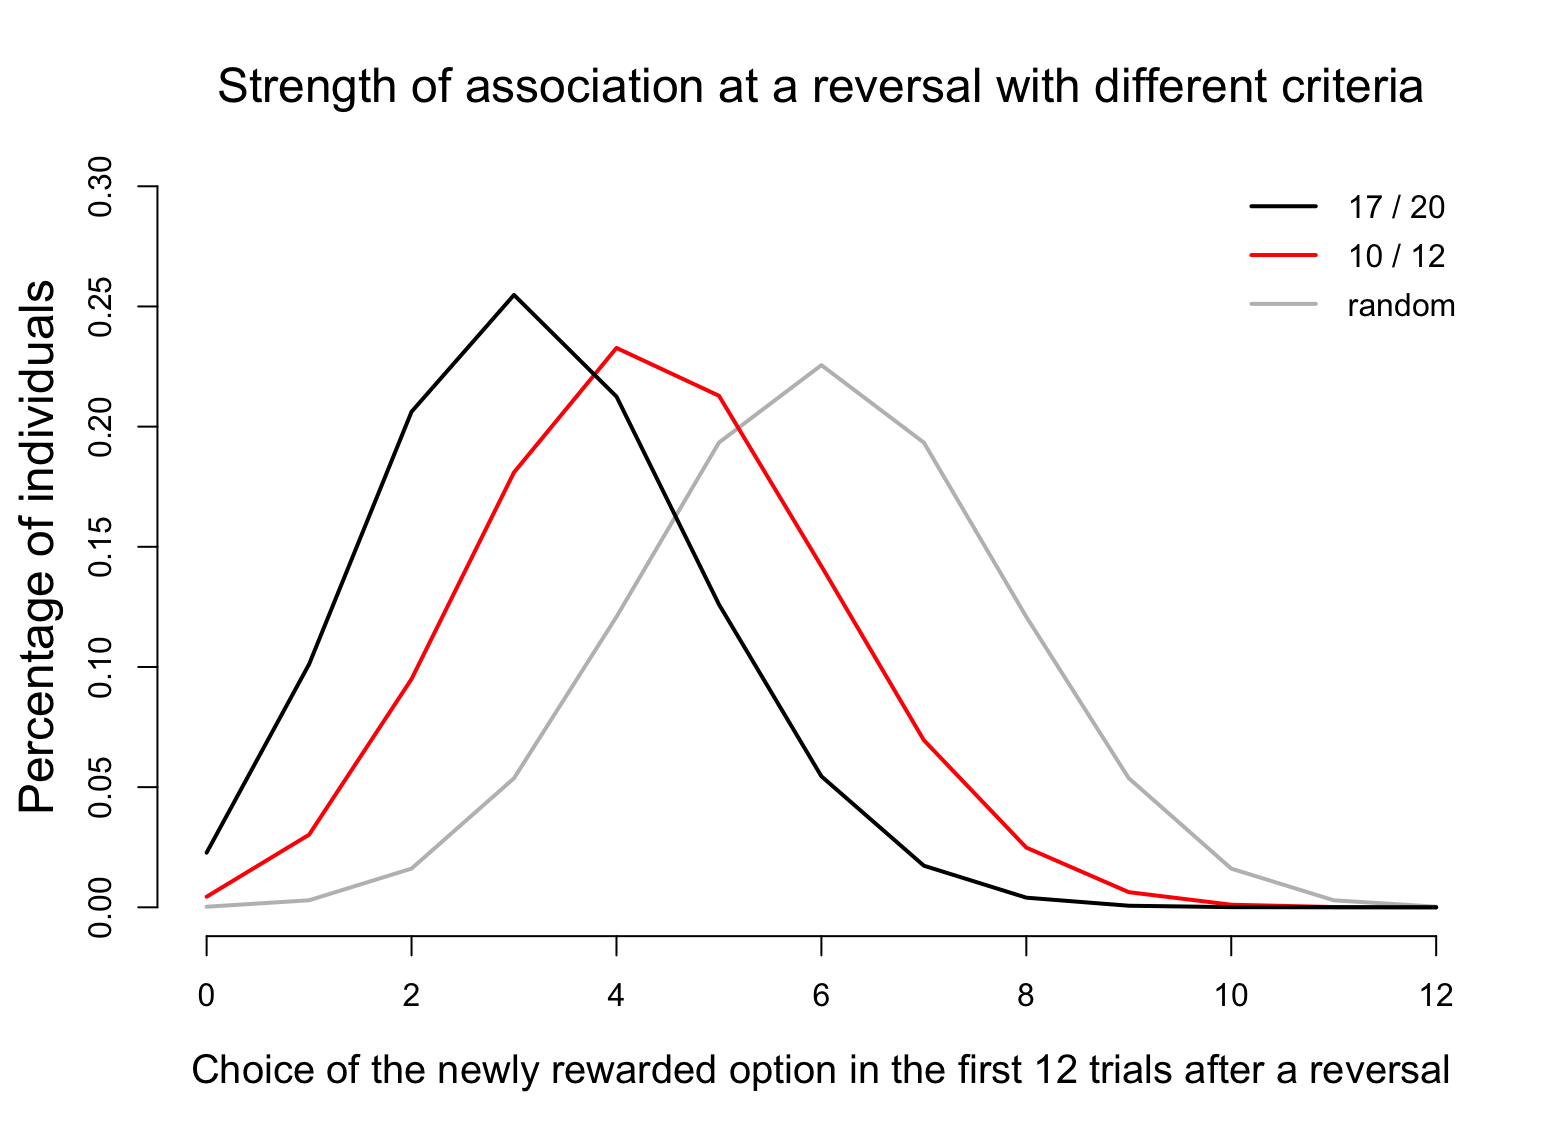
\includegraphics[width=0.6\linewidth,height=\textheight,keepaspectratio]{m1Fig_ReversalCriterionAssociation.png}

\textbf{Figure S2.} Individuals form strong enough preferences using the
10/12 passing criterion as indicated by the fact that they are unlikely
to pass in the first 12 trials of their next reversal (red line). These
individuals would take longer to switch their preference than
individuals who have no preference (gray line), and they would be
slightly faster at switching their preference than individuals who
formed their previous association using the 17/20 criterion (black
line).

\subsection{S2 - Determining after which reversal an individual has
completed the experiment: serial reversal passing
criterion}\label{s2---determining-after-which-reversal-an-individual-has-completed-the-experiment-serial-reversal-passing-criterion}

Data from previous serial reversal experiments suggests that individuals
who go through multiple reversals will end up with a performance that is
similar to the individuals who needed the fewest trials on the first
reversal (Logan et al., 2022; Lucon-Xiccato \& Bisazza, 2014). This
suggests that the manipulation changes individuals within their natural
range of variation rather than pushing them to new limits. This means
that we can use the performance of the fastest individuals in the first
reversal to set the criterion for passing the serial reversal
experiment. Accordingly, we can only set the serial reversal passing
criterion after the data from the first reversal begins to become
available. Some species might already have data from previous studies on
reversal learning, however it is important to set the passing criterion
for this experiment using this particular setup. Therefore, the
criterion must be established from scratch for each species using this
setup.

\textbf{The serial reversal passing criterion:} reach the reversal
passing criterion (10 out of 12 trials correct) in X trials or fewer in
two consecutive reversals.

X = the number of trials required that marks the fastest 20\% of
individuals in the first reversal. For example, if you test 20
individuals, the number of trials for the 4th fastest individual will be
the criterion. For 10 individuals, use the number of trials for the 2nd
fastest individual. The fastest 20\% was validated using the grackle
data (Logan et al., 2022): it aligns with the one sigma rule from a
normal distribution, indicating the percentage of individuals who are
faster than the mean number of trials minus one standard deviation. If
more than 20\% of individuals reach this number of trials in their first
reversal (because there might be a tie), choose the next fastest number
of trials to pass. Particularly near the beginning of the experiment, it
will be important to set the passing criterion to a lower number to
ensure that individuals will be overtrained rather than undertrained.

As the data for additional individuals becomes available, this number
can change accordingly. If the number changes across the experiment, we
will check whether any currently participating individuals would have
already passed according to this criterion and end their experiment.

Individuals need to meet this criterion in two consecutive reversals to
pass the serial reversal experiment to ensure that their behavior is
consistent and that their speedy performance did not occur by chance.
Previous serial reversal experiments show that reversal performance
plateaus after a certain number of reversals (e.g., 6-8 reversals in
great-tailed grackles Logan et al., 2022). If individuals show no
consistent improvement after 12 reversals and have not yet met the
serial reversal passing criterion, they will be excluded from the
experiment. We will plan to start with many more individuals than the
minimum sample size to allow for potential drop outs.

We do not expect that the serial reversal manipulation will introduce
new negative effects because the passing criterion is set such that the
manipulated individuals are only as fast as the fastest 20\% of tested
individuals. This means that we are not introducing an unnatural amount
of flexibility because we are not making any individuals more flexible
than what already exists in their population.

There will be individual variation in terms of baseline flexibility
before the manipulation such that the flexibility training might
influence individuals differently. For example, individuals who are
already flexible before the manipulation will not benefit much from the
manipulation, while the less flexible individuals will benefit more.
Individuals who are already flexible and pass the serial reversals in
fewer reversals will still meet the experiment's passing criterion and
be considered to have completed the manipulation, even if they did not
improve. Baseline flexibility differences could also be reflected in
their pre-manipulation success measures (i.e., individuals with high
baseline flexibility might already be successful before the
manipulation) if these success measures relate to flexibility. Our
statistical models account for these baseline individual differences in
success as they might relate to performance on the flexibility
manipulation because they include an interaction between the intercept
(the value at which individuals start) and slope (by how much they
change).

\subsection{S3 - Planned Sample}\label{s3---planned-sample}

For each population, depending on the response variable, we ran separate
power analyses to determine the planned sample size (see Analysis Plan).
For each population, we will aim to reach the minimum sample size
required to detect the expected effects of the intervention on the
response variables. However, given the difficulties of working with wild
individuals, there might be instances where we might not reach a
particular target. In such a case, we will interpret the result in light
of the power that the particular sample size provides, as indicated by
the power analyses. The minimum sample size depends on whether the
intervention is performed as a within-subject design (higher power),
measuring the response for the same individuals before and after the
intervention, or whether it is performed as a between-subjects design,
where half the individuals are randomly assigned to the intervention
group. In addition, it will depend on whether the response variable has
a binary or a continuous outcome (higher power), and in the latter case
whether the measure is open-ended (lower power) and therefore
individuals will show a large range of values (e.g., dispersal
distance).

We will stop collecting data for the flexibility manipulation experiment
when a buffer above the minimum sample size is reached or when the
season in which the minimum sample size is reached comes to an end, or
when the minimum sample sizes for the success measures have been
reached. When conducting the manipulation experiment, it is important to
aim to test more than the minimum number of individuals because some
might not have data in the post-intervention stage.

\section{S4 - Power analyses simulations and model
code}\label{s4---power-analyses-simulations-and-model-code}

We run analyses in R {[}current version 4.5.0; R Core Team (2017){]}
using the following R packages: rethinking (McElreath, 2020a), rstan
(Stan Development Team, 2020), cmdstanr (Gabry \& Češnovar, 2022), knitr
(Xie, 2018), and irr (Gamer et al., 2012). We describe below the
Bayesian models we developed to address each of the specific research
questions. All Bayesian models were developed using McElreath (2020b) as
a guide. Code for running these models is available in supplementary
materials S4.

\subsection{J.Q1 Do jay populations in human modified areas differ in
baseline behavioral flexibility compared to populations in natural
areas?}\label{j.q1-do-jay-populations-in-human-modified-areas-differ-in-baseline-behavioral-flexibility-compared-to-populations-in-natural-areas-2}

\textbf{The model}

We used the reversal learning Bayesian model in Logan CJ et al. (2020)
to simulate and analyze population differences in reversal learning, and
calculate our ability to detect differences between populations. The
model ``accounts for every choice made in the reversal learning
experiment and updates the probability of choosing either option after
the choice was made depending on whether that choice contained a food
reward or not. It does this by updating three main components for each
choice: an attraction score, a learning rate (\(\phi\)), and a rate of
deviating from learned attractions (\(\lambda\))'' (Logan CJ et al.,
2020).

\textbf{\emph{Equation 1 (attraction and \(\phi\)):}}
\(A_{i,j, t+1} = (1-\phi_j) A_{i,j,t} + \phi_j \pi_{i,j,t}\)

Equation 1 ``tells us how attractions to different behavioral options
\(A_{i,j, t+1}\) (i.e., how preferable option \(i\) is to the bird \(j\)
at time \(t+1\)) change over time as a function of previous attractions
\(A_{i ,j, t}\) and recently experienced payoffs \(\pi_{i,j,t}\) (i.e.,
whether they received a reward in a given trial or not). Attraction
scores thus reflect the accumulated learning history up to this point.
The (bird-specific) parameter \(\phi_j\) describes the weight of recent
experience. The higher the value of \(\phi_j\), the faster the bird
updates their attraction. It thus can be interpreted as the
\emph{learning or updating rate of an individual}. A value of
\(\phi_j = 0.04\), for example, means that receiving a single reward for
one of the two options will shift preferences by 0.02 from initial
0.5-0.5 attractions, a value of \(\phi_j = 0.06\) will shift preferences
by 0.03 and so on'' (Blaisdell et al., 2021).

\textbf{\emph{Equation 2 (\(\lambda\)):}}
\(P(i)_{t+1} = \frac{\exp(\lambda_j A_{i, j, t})}{\sum\limits_{m=1}^{2}\exp(\lambda_j A_{m, j, t})}.\)

Equation 2 ``expresses the probability an individual \(j\) chooses
option \(i\) in the next round, \(t+1\), based on the latent
attractions. The parameter \(\lambda_j\) represents the \emph{rate of
deviating from learned attractions} of an individual (also called
inverse temperature). It controls how sensitive choices are to
differences in attraction scores. As \(\lambda_j\) gets larger, choices
become more deterministic, as it gets smaller, choices become more
exploratory (random choice if \(\lambda_j = 0\)). For instance, if an
individual has a 0.6-0.4 preference for option A, a value of
\(\lambda_j = 3\) means they choose A 65\% of the time, a value of
\(\lambda_j = 10\) means they choose A 88\% of the time and a value of
\(\lambda_j = 0.5\) means they choose A only 53\% of the time''
(Blaisdell et al., 2021).

We used the \(\phi_j\) and \(\lambda_j\) values as the response variable
in the Bayesian model to examine whether there were differences in
flexibility between the habitats:

y \textasciitilde{} \(\alpha\){[}habitat{]}

y is the response variable (\(\phi_j\) and \(\lambda_j\), which are
extracted from the correct and incorrect choices in the serial
reversals). There is one intercept, \(\alpha\), per habitat (suburban or
natural) and we will estimate the habitat's average and standard
deviation of the response variable.

\textbf{Power analysis}

Simulations using bespoke Bayesian models in Logan CJ et al. (2020) (the
same model structure we use here) showed a high likelihood of detecting
differences with a minimum sample size of 15 when mean differences in
phi were at least 0.01 and mean differences in lambda at least 3.

\textbf{Run this model on the actual data}

Run the code below to determine whether there were differences between
the two habitats in their phi and lambda flexibility measures.

\paragraph{J.Q2 Are disturbance-resiliant jays more flexible than
disturbance-resistant
jays?}\label{j.q2-are-disturbance-resiliant-jays-more-flexible-than-disturbance-resistant-jays-1}

\textbf{The model}

Same as in J.Q1 above.

\textbf{Power analysis}

Same as in J.Q1 above.

\paragraph{J.Q3 More flexible = use more
microhabitats?}\label{j.q3-more-flexible-use-more-microhabitats-2}

\textbf{The model}

\emph{Bayesian model with a normal distribution:}

habitatuse \textasciitilde{} \(\alpha\){[}ind{]} +
\(\beta\){[}ind{]}*before

habitatuse is the response variable: the total number of different
microhabitats used per individual. There will be one intercept,
\(\alpha\), and one slope \(\beta\) per individual, which will be
estimated for the two conditions, before (and after) the manipulation.
ID is nested within condition as a random effect because there is more
than one data point per individual: each individual has a data point in
the before condition and in the after condition. A normal distribution
was used because the response variable is a sum without an expected skew
to the curve (see Figure 10.6 in McElreath, 2020b). The Bayesian model
was developed using McElreath (2020b) as a guide.

\textbf{Power analysis}

We estimated our power to detect differences between conditions at
different sample sizes and with different mean changes in the proportion
of different microhabitats used per individual in the before vs.~after
conditions (Figure 11). We simulated the proportion of habitats used for
different sample sizes of individuals before and after the flexibility
manipulation. We analyzed these simulated data with the model we will
use to analyze the actual data, estimating the change in the proportion
of habitats used between the before and after conditions. From the
posterior estimates of the model, we extracted both the mean change as
well as the ratio of the posterior estimates that were below zero.

If the mean ratio of estimates below zero is close to 0.5, the model
assumes that the change in the proportion of habitats used before the
flexibility manipulation is similar to after. If the ratio is close to
zero, the model assumes individuals have changed their behavior. For
changes in the proportion of habitats used smaller than 0.15 (standard
deviation=0.2) or 0.1 (SD=0.1), models are likely to assume that no
changes occurred even with large sample sizes. If the change in the
proportion of habitats used before the flexibility manipulation
vs.~after is 0.15 with a standard deviation of 0.2, on average 94\% of
the posterior of the model based on a sample size of 20 individuals will
be larger than zero (93\% with a standard deviation of 0.1). This means
that the model is quite certain there is a difference that is larger
than zero. In addition, only four of the 30 models for a sample size of
20 at the mean change of 0.15 have a ratio larger than 0.3, meaning that
the risk of having a false negative is not very likely.

In general, with sample sizes at or above 20 and mean changes in the
proportion of habitats used at 0.1 or larger, it is highly likely that
the model will indicate that individuals have changed their behavior.
Mean changes below 0.1 can still be detected, however there is a higher
risk that there will be a false negative and this risk is independent of
sample size.

With small mean changes in the response variable, some individuals might
not increase or even decrease their response after the manipulation
because there is variation around the mean change in individual
responses. With small sample sizes, there is a risk that only
individuals who did not clearly increase their response will be studied,
whereas larger sample sizes are more likely to include a wider spectrum
of individuals.

To estimate the risk of detecting false positives, we set the mean
change in the proportion of habitats used to zero so there was no change
between the before and after conditions. As expected, the average ratio
of estimates below zero is close to but below 0.5 and independent of
sample size. The estimates went generally below 0.5 because the maximum
number of habitats used was set to 10 and we had a condition where
individuals before the manipulation used a mean of 7 habitats.
Accordingly, if individuals randomly either increase or decrease their
number of habitats used, decreases will be more severe because
individuals can only increase by 3 habitats, but potentially decrease by
6 habitats. With a sample size of 20, 27\% have a ratio smaller than
0.3, meaning that the risk of having a false positive is high. The risk
would be lower if the variation among individuals was lower than what we
assumed (the standard deviation of the mean change in number of habitats
was 0.2, which is a conservative estimate).

~

\textbf{Figure 11.} Risk of false positives and false negatives
depending on sample and effect sizes. Curves of the mean ratio of
estimates below zero (vertical lines show the minimum and maximum
ratios), which illustrates the power we have to detect differences
between conditions at different sample sizes. Across all models, the
standard deviation of the mean change in proportion of habitats used was
0.2 (A) or 0.1 (B). A mean change in proportion of habitats of 0.3 is
associated with a difference of 3 habitats (when the maximum number of
habitats is 10). The curves show the model estimates as the effect
increases (larger changes in the mean proportion time spent after versus
before on the x-axis) for different potential sample sizes (10-60,
illustrated by different colors). When there is no change (x value of
zero), estimates suggest that, as expected, half of the estimates are
below zero because the before and after conditions are not different
from each other. As the change increases, the estimates decrease because
models are able to reliably tell that the before and after conditions
differ from each other.

~

\textbf{Run this model on the actual data}

Run the code below to determine whether there were differences between
the before and after conditions in the proportion of microhabitats used.
Only count that a microhabitat was used if the individual had at least
5\% of their data points there. This prevents a microhabitat from being
counted even if an individual was simply moving through it, and
therefore not necessarily using it.

\paragraph{J.Q4 More flexible = more food
types?}\label{j.q4-more-flexible-more-food-types-2}

\textbf{The model}

\emph{Bayesian model with a normal distribution:}

y \textasciitilde{} \(\alpha\){[}ind{]} + \(\beta\){[}ind{]}*before

y is the response variable: the total number of different food types
taken per individual. There will be one intercept, \(\alpha\), and one
slope \(\beta\) per individual, which will be estimated for the two
conditions, before (and after) the manipulation. ID is nested within
condition as a random effect because there is more than one data point
per individual: each individual has a data point in the before condition
and in the after condition. A normal distribution was used because the
response variable is a sum without an expected skew to the curve (see
Figure 10.6 in McElreath, 2020b). The Bayesian model was developed using
McElreath (2020b) as a guide.

\textbf{Power analysis}

We estimated our power to detect differences between conditions at
different sample sizes and with different mean changes in the total
number of different food types taken per individual in the before
vs.~after conditions (Figure 12). We simulated the number of food types
taken for different sample sizes of individuals before and after the
flexibility manipulation. We analyzed these simulated data with the
model we will use to analyze the actual data, estimating the change in
the number of food types taken between the before and after conditions.
From the posterior estimates of the model, we extracted both the mean
change as well as the ratio of the posterior estimates that were below
zero.

If the mean ratio of estimates below zero is close to 0.5, the model
assumes that the change in the number of food types taken before the
flexibility manipulation is similar to after. If the ratio is close to
zero, the model assumes individuals have changed their behavior. For
changes in the number of food types taken smaller than 1, models are
likely to assume that no changes occurred even with large sample sizes.
If the change in the number of food types taken before the flexibility
manipulation vs.~after is 1 with a standard deviation of 2, on average
99.96\% of the posterior of the model based on a sample size of 20
individuals will be larger than zero. This means that the model is quite
certain there is a difference that is larger than zero. In addition,
none of the 30 models for a sample size of 20 at the mean change of 1
have a ratio larger than 0.3, meaning that the risk of having a false
negative is not very likely.

In general, with sample sizes at or above 20 and mean changes in the
number of food types taken at 1 or larger, it is likely that the model
will indicate that individuals have changed their behavior. Mean changes
below 1 can still be detected, however there is a higher risk that there
will be a false negative and this risk is independent of sample size.
For example, 17\% of the models for a sample size of 20 at the mean
change of 0.5 have a ratio larger than 0.3, meaning there is a risk of
having a false negative.

With small mean changes in the response variable, some individuals might
not increase or even decrease their response after the manipulation
because there is variation around the mean change in individual
responses. With small sample sizes, there is a risk that only
individuals who did not clearly increase their response will be studied,
whereas larger sample sizes are more likely to include a wider spectrum
of individuals.

To estimate the risk of detecting false positives, we set the mean
change in the number of food types taken to zero so there was no change
between the before and after conditions. As expected, the average ratio
of estimates below zero is close to 0.5 and independent of sample size.
With a sample size of 20, 30\% have a ratio smaller than 0.3, meaning
that the risk of having a false positive is high. The risk would be
lower if the variation among individuals was lower than what we assumed
(the standard deviation of the mean change in number of foods was 2,
which is a conservative estimate).

~

\textbf{Figure 12.} Risk of false positives and false negatives
depending on sample and effect sizes. Curves of the mean ratio of
estimates below zero (vertical lines show the minimum and maximum
ratios), which illustrates the power we have to detect differences
between conditions at different sample sizes. Across all models, the
standard deviation of the mean change in number of food types taken was
2 (A) or 1 (B), and the number of food types taken before the
flexibility manipulation was 6.5. A mean change in proportion of
habitats of 0.3 is associated with a difference of 3 habitats (when the
maximum number of habitats is 10). The curves show the model estimates
as the effect increases (larger changes in the mean proportion time
spent after versus before on the x-axis) for different potential sample
sizes (10-60, illustrated by different colors). When there is no change
(x value of zero), estimates suggest that, as expected, half of the
estimates are below zero because the before and after conditions are not
different from each other. As the change increases, the estimates
decrease because models are able to reliably tell that the before and
after conditions differ from each other.

~

\textbf{Run this model on the actual data}

Run the code to determine whether there were differences between the
before and after conditions in the number of food types taken.

\section*{\texorpdfstring{\textbf{REFERENCES}}{REFERENCES}}\label{references}
\addcontentsline{toc}{section}{\textbf{REFERENCES}}

\phantomsection\label{refs}
\begin{CSLReferences}{1}{0}
\bibitem[\citeproctext]{ref-alberti2015eco}
Alberti, M. (2015). Eco-evolutionary dynamics in an urbanizing planet.
\emph{Trends in Ecology \& Evolution}, \emph{30}(2), 114--126.
\url{https://doi.org/10.1016/j.tree.2014.11.007}

\bibitem[\citeproctext]{ref-bebus2016associative}
Bebus, S. E., Small, T. W., Jones, B. C., Elderbrock, E. K., \& Schoech,
S. J. (2016). Associative learning is inversely related to reversal
learning and varies with nestling corticosterone exposure. \emph{Animal
Behaviour}, \emph{111}, 251--260.

\bibitem[\citeproctext]{ref-blair1996land}
Blair, R. B. (1996). Land use and avian species diversity along an urban
gradient. \emph{Ecological Applications}, \emph{6}(2), 506--519.

\bibitem[\citeproctext]{ref-blaisdell2021causal}
Blaisdell, A., Seitz, B., Rowney, C., Folsom, M., MacPherson, M.,
Deffner, D., \& Logan, C. J. (2021). \emph{Do the more flexible
individuals rely more on causal cognition? Observation versus
intervention in causal inference in great-tailed grackles (version 5 of
this preprint has been peer reviewed and recommended by peer community
in ecology {[}https://doi.org/10.24072/pci.ecology.100076{]})}.
\url{https://doi.org/10.31234/osf.io/z4p6s}

\bibitem[\citeproctext]{ref-bond_serial_2007}
Bond, A. B., Kamil, A. C., \& Balda, R. P. (2007). Serial reversal
learning and the evolution of behavioral flexibility in three species of
{North} {American} corvids (\emph{{Gymnorhinus} cyanocephalus},
\emph{{Nucifraga} columbiana}, \emph{{Aphelocoma} californica}).
\emph{Journal of Comparative Psychology}, \emph{121}(4), 372--379.
\url{https://doi.org/10.1037/0735-7036.121.4.372}

\bibitem[\citeproctext]{ref-chejanovski2017experimental}
Chejanovski, Z. A., Avilés-Rodrı́guez, K. J., Lapiedra, O., Preisser, E.
L., \& Kolbe, J. J. (2017). An experimental evaluation of foraging
decisions in urban and natural forest populations of anolis lizards.
\emph{Urban Ecosystems}, \emph{20}(5), 1011--1018.
\url{https://doi.org/10.1007/s11252-017-0654-5}

\bibitem[\citeproctext]{ref-ciani1986intertroop}
Ciani, A. C. (1986). Intertroop agonistic behavior of a feral rhesus
macaque troop ranging in town and forest areas in india.
\emph{Aggressive Behavior}, \emph{12}(6), 433--439.
\url{https://doi.org/10.1002/1098-2337(1986)12:6\%3C433::AID-AB2480120606\%3E3.0.CO;2-C}

\bibitem[\citeproctext]{ref-curry2017california}
Curry, R., Townsend Peterson, A., \& Langen, T. (2017). \emph{California
scrub-jay (aphelocoma californica), birds of north america}.

\bibitem[\citeproctext]{ref-daniel2020serial}
Daniel, M. M., \& Schluessel, V. (2020). Serial reversal learning in
freshwater stingrays (potamotrygon motoro). \emph{Animal Cognition},
\emph{23}(1), 109--119. \url{https://doi.org/10.1007/s10071-019-01321-x}

\bibitem[\citeproctext]{ref-emery2004mentality}
Emery, N. J., \& Clayton, N. S. (2004). The mentality of crows:
Convergent evolution of intelligence in corvids and apes.
\emph{Science}, \emph{306}(5703), 1903--1907.

\bibitem[\citeproctext]{ref-federspiel2017adjusting}
Federspiel, I. G., Garland, A., Guez, D., Bugnyar, T., Healy, S. D.,
Güntürkün, O., \& Griffin, A. S. (2017). Adjusting foraging strategies:
A comparison of rural and urban common mynas (acridotheres tristis).
\emph{Animal Cognition}, \emph{20}(1), 65--74.
\url{https://doi.org/10.1007/s10071-016-1045-7}

\bibitem[\citeproctext]{ref-cmdstanr}
Gabry, J., \& Češnovar, R. and. (2022). \emph{Cmdstanr: R interface to
'CmdStan'}. \url{https://mc-stan.org/cmdstanr/}

\bibitem[\citeproctext]{ref-galbraith2015supplementary}
Galbraith, J. A., Beggs, J. R., Jones, D. N., \& Stanley, M. C. (2015).
Supplementary feeding restructures urban bird communities.
\emph{Proceedings of the National Academy of Sciences}, \emph{112}(20),
E2648--E2657.

\bibitem[\citeproctext]{ref-gamer2012package}
Gamer, M., Lemon, J., Gamer, M. M., Robinson, A., \& Kendall's, W.
(2012). Package {``irr.''} \emph{Various Coefficients of Interrater
Reliability and Agreement}, \emph{22}.

\bibitem[\citeproctext]{ref-goldewijk2001estimating}
Goldewijk, K. K. (2001). Estimating global land use change over the past
300 years: The HYDE database. \emph{Global Biogeochemical Cycles},
\emph{15}(2), 417--433. \url{https://doi.org/10.1029/1999GB001232}

\bibitem[\citeproctext]{ref-greggor2021pre}
Greggor, A. L., Masuda, B., Gaudioso-Levita, J. M., Nelson, J. T.,
White, T. H., Shier, D. M., Farabaugh, S. M., \& Swaisgood, R. R.
(2021). Pre-release training, predator interactions and evidence for
persistence of anti-predator behavior in reintroduced alal{ā}, hawaiian
crow. \emph{Global Ecology and Conservation}, \emph{28}, e01658.
\url{https://doi.org/10.1016/j.gecco.2021.e01658}

\bibitem[\citeproctext]{ref-greig2017winter}
Greig, E. I., Wood, E. M., \& Bonter, D. N. (2017). Winter range
expansion of a hummingbird is associated with urbanization and
supplementary feeding. \emph{Proceedings of the Royal Society B:
Biological Sciences}, \emph{284}(1852).

\bibitem[\citeproctext]{ref-grinnell1917niche}
Grinnell, J. (1917). The niche-relationships of the california thrasher.
\emph{The Auk}, \emph{34}(4), 427--433.
\url{https://doi.org/10.2307/4072271}

\bibitem[\citeproctext]{ref-jolly2018out}
Jolly, C. J., Kelly, E., Gillespie, G. R., Phillips, B., \& Webb, J. K.
(2018). Out of the frying pan: Reintroduction of toad-smart northern
quolls to southern kakadu national park. \emph{Austral Ecology},
\emph{43}(2), 139--149. \url{https://doi.org/10.1111/aec.12551}

\bibitem[\citeproctext]{ref-lapiedra2017urbanization}
Lapiedra, O., Chejanovski, Z., \& Kolbe, J. J. (2017). Urbanization and
biological invasion shape animal personalities. \emph{Global Change
Biology}, \emph{23}(2), 592--603.

\bibitem[\citeproctext]{ref-lee2021animal}
Lee, V. E., \& Thornton, A. (2021). Animal cognition in an urbanised
world. \emph{Frontiers in Ecology and Evolution}, \emph{9}, 120.
\url{https://doi.org/10.3389/fevo.2021.633947}

\bibitem[\citeproctext]{ref-liu2020high}
Liu, X., Huang, Y., Xu, X., Li, X., Li, X., Ciais, P., Lin, P., Gong,
K., Ziegler, A. D., Chen, A., et al. (2020).
High-spatiotemporal-resolution mapping of global urban change from 1985
to 2015. \emph{Nature Sustainability}, 1--7.
\url{https://doi.org/10.1038/s41893-020-0521-x}

\bibitem[\citeproctext]{ref-liu2016learning}
Liu, Y., Day, L. B., Summers, K., \& Burmeister, S. S. (2016). Learning
to learn: Advanced behavioural flexibility in a poison frog.
\emph{Animal Behaviour}, \emph{111}, 167--172.
\url{https://doi.org/10.1016/j.anbehav.2015.10.018}

\bibitem[\citeproctext]{ref-logan2016flexibilityproblem}
Logan, C. J. (2016). Behavioral flexibility and problem solving in an
invasive bird. \emph{PeerJ}, \emph{4}, e1975.
\url{https://doi.org/10.7717/peerj.1975}

\bibitem[\citeproctext]{ref-logan2022flexmanip}
Logan, C., Blaisdell, A., Johnson-Ulrich, Z., Lukas, D., MacPherson, M.,
Seitz, B., Sevchik, A., \& McCune, K. (2022). Behavioral flexibility is
manipulatable and it improves flexibility and problem solving in a new
context. \emph{EcoEvoRxiv}.
https://doi.org/\url{https://doi.org/10.32942/osf.io/5z8xs}

\bibitem[\citeproctext]{ref-logan2020xpop}
Logan, CJ, McCune, KB, Breen, A, Chen, N, \& Lukas, D. (2020).
Implementing a rapid geographic range expansion - the role of behavior
and habitat changes. \emph{In Principle Acceptance by PCI Ecology of the
Version on 6 Oct 2020}.
\url{http://corinalogan.com/Preregistrations/gxpopbehaviorhabitat.html}

\bibitem[\citeproctext]{ref-logan2023flexmanippcj}
Logan, C., Lukas, D., Blaisdell, A., Johnson-Ulrich, Z., MacPherson, M.,
Seitz, B., Sevchik, A., \& McCune, K. (2023). Behavioral flexibility is
manipulable and it improves flexibility and innovativeness in a new
context. \emph{Peer Community Journal}, \emph{3}.
\url{https://doi.org/10.24072/pcjournal.284}

\bibitem[\citeproctext]{ref-logan2025behavioral}
Logan, C., Lukas, D., Geng, X., Hardy, K., LeGrande, C., Marfori, Z.,
MacPherson, M., Rowney, C., Smith, C., \& McCune, K. (2025). Behavioral
flexibility is related to foraging, but not social or habitat use
behaviors, in a species that is rapidly expanding its range. \emph{Peer
Community Journal}, \emph{5}.

\bibitem[\citeproctext]{ref-lucon2014discrimination}
Lucon-Xiccato, T., \& Bisazza, A. (2014). Discrimination reversal
learning reveals greater female behavioural flexibility in guppies.
\emph{Biology Letters}, \emph{10}(6), 20140206.
\url{https://doi.org/10.1098/rsbl.2014.0206}

\bibitem[\citeproctext]{ref-mackintosh1968factors}
Mackintosh, N., Mcgonigle, B., \& Holgate, V. (1968). Factors underlying
improvement in serial reversal learning. \emph{Canadian Journal of
Psychology/Revue Canadienne de Psychologie}, \emph{22}(2), 85.
\url{https://doi.org/10.1037/h0082753}

\bibitem[\citeproctext]{ref-mccune2019captive}
McCune, K. B., Jablonski, P., Lee, S., \& Ha, R. R. (2019). Captive jays
exhibit reduced problem-solving performance compared to wild
conspecifics. \emph{Royal Society Open Science}, \emph{6}(1), 181311.

\bibitem[\citeproctext]{ref-mccune2022social}
McCune, K. B., Valente, J. J., Jablonski, P. G., Lee, S., \& Ha, R. R.
(2022). Social behavior mediates the use of social and personal
information in wild jays. \emph{Scientific Reports}, \emph{12}(1), 2494.

\bibitem[\citeproctext]{ref-mccune2020spaceuse}
McCune, KB, Folsom, M, Ross, C, Bergeron, L, \& Logan, C. (2020). Does
great-tailed grackle space use behavior reflect individual differences
in exploration? \emph{In Principle Acceptance by PCI Ecology of the
Version on 23 Sep 2020}.
\url{http://corinalogan.com/Preregistrations/gspaceuse.html}

\bibitem[\citeproctext]{ref-mccune2023using}
McCune, K., Blaisdell, A., Johnson-Ulrich, Z., Sevchik, A., Lukas, D.,
MacPherson, M., Seitz, B., \& Logan, C. J. (2023). Using repeatability
of performance within and across contexts to validate measures of
behavioral flexibility. \emph{PeerJ}, \emph{11}, e15773.

\bibitem[\citeproctext]{ref-rethinking2020}
McElreath, R. (2020a). \emph{Rethinking: Statistical rethinking book
package}.

\bibitem[\citeproctext]{ref-mcelreath2020statistical}
McElreath, R. (2020b). \emph{Statistical rethinking: A bayesian course
with examples in r and stan}. Chapman; Hall/CRC.

\bibitem[\citeproctext]{ref-midford2000social}
Midford, P. E., Hailman, J. P., \& Woolfenden, G. E. (2000). Social
learning of a novel foraging patch in families of free-living florida
scrub-jays. \emph{Animal Behaviour}, \emph{59}(6), 1199--1207.

\bibitem[\citeproctext]{ref-mikhalevich_is_2017}
Mikhalevich, I., Powell, R., \& Logan, C. (2017). Is behavioural
flexibility evidence of cognitive complexity? {How} evolution can inform
comparative cognition. \emph{Interface Focus}, \emph{7}(3), 20160121.
\url{https://doi.org/10.1098/rsfs.2016.0121}

\bibitem[\citeproctext]{ref-moseby2016harnessing}
Moseby, K. E., Blumstein, D. T., \& Letnic, M. (2016). Harnessing
natural selection to tackle the problem of prey na{ı̈}vet{é}.
\emph{Evolutionary Applications}, \emph{9}(2), 334--343.
\url{https://doi.org/10.1111/eva.12332}

\bibitem[\citeproctext]{ref-moseby2012can}
Moseby, K. E., Cameron, A., \& Crisp, H. A. (2012). Can predator
avoidance training improve reintroduction outcomes for the greater bilby
in arid australia? \emph{Animal Behaviour}, \emph{83}(4), 1011--1021.
\url{https://doi.org/10.1016/j.anbehav.2012.01.023}

\bibitem[\citeproctext]{ref-peterson2011ecological}
Peterson, A. T., Soberón, J., Pearson, R. G., Anderson, R. P.,
Martı́nez-Meyer, E., Nakamura, M., \& Araújo, M. B. (2011). Ecological
niches and geographic distributions (MPB-49). In \emph{Ecological niches
and geographic distributions (MPB-49)}. Princeton University Press.
\url{https://doi.org/10.1515/9781400840670}

\bibitem[\citeproctext]{ref-rcoreteam}
R Core Team. (2017). \emph{R: A language and environment for statistical
computing}. R Foundation for Statistical Computing.
\url{https://www.R-project.org}

\bibitem[\citeproctext]{ref-rice2003ecological}
Rice, N. H., Martinez-Meyer, E., \& Peterson, A. T. (2003). Ecological
niche differentiation in the aphelocoma jays: A phylogenetic
perspective. \emph{Biological Journal of the Linnean Society},
\emph{80}(3), 369--383.

\bibitem[\citeproctext]{ref-ross2019reversing}
Ross, A. K., Letnic, M., Blumstein, D. T., \& Moseby, K. E. (2019).
Reversing the effects of evolutionary prey naivet{é} through controlled
predator exposure. \emph{Journal of Applied Ecology}, \emph{56}(7),
1761--1769. \url{https://doi.org/10.1111/1365-2664.13406}

\bibitem[\citeproctext]{ref-shaw2015wild}
Shaw, R. C., Boogert, N. J., Clayton, N. S., \& Burns, K. C. (2015).
Wild psychometrics: Evidence for `general'cognitive performance in wild
new zealand robins, petroica longipes. \emph{Animal Behaviour},
\emph{109}, 101--111.

\bibitem[\citeproctext]{ref-shawkey2004brood}
Shawkey, M. D., Bowman, R., \& Woolfenden, G. E. (2004). Why is brood
reduction in florida scrub-jays higher in suburban than in wildland
habitats? \emph{Canadian Journal of Zoology}, \emph{82}(9), 1427--1435.

\bibitem[\citeproctext]{ref-snell2019behaviour}
Snell-Rood, E. C., \& Steck, M. K. (2019). Behaviour shapes
environmental variation and selection on learning and plasticity: Review
of mechanisms and implications. \emph{Animal Behaviour}, \emph{147},
147--156.

\bibitem[\citeproctext]{ref-sol2002behavioural}
Sol, D., Timmermans, S., \& Lefebvre, L. (2002). Behavioural flexibility
and invasion success in birds. \emph{Animal Behaviour}, \emph{63}(3),
495--502. \url{https://doi.org/10.1006/anbe.2001.1953}

\bibitem[\citeproctext]{ref-rstan}
Stan Development Team. (2020). \emph{{RStan}: The {R} interface to
{Stan}}. \url{http://mc-stan.org/}

\bibitem[\citeproctext]{ref-strang2014serial}
Strang, C. G., \& Sherry, D. F. (2014). Serial reversal learning in
bumblebees (bombus impatiens). \emph{Animal Cognition}, \emph{17}(3),
723--734. \url{https://doi.org/10.1007/s10071-013-0704-1}

\bibitem[\citeproctext]{ref-tetzlaff2019effects}
Tetzlaff, S. J., Sperry, J. H., \& DeGregorio, B. A. (2019). Effects of
antipredator training, environmental enrichment, and soft release on
wildlife translocations: A review and meta-analysis. \emph{Biological
Conservation}, \emph{236}, 324--331.
\url{https://doi.org/10.1016/j.biocon.2019.05.054}

\bibitem[\citeproctext]{ref-tuomainen2011behavioural}
Tuomainen, U., \& Candolin, U. (2011). Behavioural responses to
human-induced environmental change. \emph{Biological Reviews},
\emph{86}(3), 640--657.

\bibitem[\citeproctext]{ref-valente2021conspecific}
Valente, J. J., LeGrande-Rolls, C. L., Rivers, J. W., Tucker, A. M.,
Fischer, R. A., \& Betts, M. G. (2021). Conspecific attraction for
conservation and management of terrestrial breeding birds: Current
knowledge and future research directions. \emph{The Condor},
\emph{123}(2), duab007. \url{https://doi.org/10.1093/ornithapp/duab007}

\bibitem[\citeproctext]{ref-vardi2022environmental}
Vardi, R., \& Berger-Tal, O. (2022). Environmental variability as a
predictor of behavioral flexibility in urban environments.
\emph{Behavioral Ecology}, \emph{33}(3), 573--581.

\bibitem[\citeproctext]{ref-veech2011effect}
Veech, J. A., Small, M. F., \& Baccus, J. T. (2011). The effect of
habitat on the range expansion of a native and an introduced bird
species. \emph{Journal of Biogeography}, \emph{38}(1), 69--77.

\bibitem[\citeproctext]{ref-wehtje2003range}
Wehtje, W. (2003). The range expansion of the great-tailed grackle
(quiscalus mexicanus gmelin) in north america since 1880. \emph{Journal
of Biogeography}, \emph{30}(10), 1593--1607.

\bibitem[\citeproctext]{ref-west2018predator}
West, R., Letnic, M., Blumstein, D. T., \& Moseby, K. E. (2018).
Predator exposure improves anti-predator responses in a threatened
mammal. \emph{Journal of Applied Ecology}, \emph{55}(1), 147--156.
\url{https://doi.org/10.1111/1365-2664.12947}

\bibitem[\citeproctext]{ref-woolfenden1996florida}
Woolfenden, G. E., \& Fitzpatrick, J. W. (1996). \emph{Florida scrub-jay
(aphelocoma coerulescens), birds of north america}.

\bibitem[\citeproctext]{ref-wright2010behavioral}
Wright, T. F., Eberhard, J. R., Hobson, E. A., Avery, M. L., \&
Russello, M. A. (2010). Behavioral flexibility and species invasions:
The adaptive flexibility hypothesis. \emph{Ethology Ecology \&
Evolution}, \emph{22}(4), 393--404.
\url{https://doi.org/10.1080/03949370.2010.505580}

\bibitem[\citeproctext]{ref-wu2011quantifying}
Wu, J., Jenerette, G. D., Buyantuyev, A., \& Redman, C. L. (2011).
Quantifying spatiotemporal patterns of urbanization: The case of the two
fastest growing metropolitan regions in the united states.
\emph{Ecological Complexity}, \emph{8}(1), 1--8.
\url{https://doi.org/10.1016/j.ecocom.2010.03.002}

\bibitem[\citeproctext]{ref-xie2018knitr}
Xie, Y. (2018). Knitr: A comprehensive tool for reproducible research in
r. In \emph{Implementing reproducible research} (pp. 3--31). Chapman;
Hall/CRC.

\end{CSLReferences}

\end{document}
